\documentclass[]{elsarticle} %review=doublespace preprint=single 5p=2 column
%%% Begin My package additions %%%%%%%%%%%%%%%%%%%
\usepackage[hyphens]{url}

  \journal{Journal of Transport Geography} % Sets Journal name


\usepackage{lineno} % add

\usepackage{graphicx}
%%%%%%%%%%%%%%%% end my additions to header

\usepackage[T1]{fontenc}
\usepackage{lmodern}
\usepackage{amssymb,amsmath}
\usepackage{ifxetex,ifluatex}
\usepackage{fixltx2e} % provides \textsubscript
% use upquote if available, for straight quotes in verbatim environments
\IfFileExists{upquote.sty}{\usepackage{upquote}}{}
\ifnum 0\ifxetex 1\fi\ifluatex 1\fi=0 % if pdftex
  \usepackage[utf8]{inputenc}
\else % if luatex or xelatex
  \usepackage{fontspec}
  \ifxetex
    \usepackage{xltxtra,xunicode}
  \fi
  \defaultfontfeatures{Mapping=tex-text,Scale=MatchLowercase}
  \newcommand{\euro}{€}
\fi
% use microtype if available
\IfFileExists{microtype.sty}{\usepackage{microtype}}{}
\bibliographystyle{elsarticle-harv}
\ifxetex
  \usepackage[setpagesize=false, % page size defined by xetex
              unicode=false, % unicode breaks when used with xetex
              xetex]{hyperref}
\else
  \usepackage[unicode=true]{hyperref}
\fi
\hypersetup{breaklinks=true,
            bookmarks=true,
            pdfauthor={},
            pdftitle={Estimating spatial availability/mismatch using singly constrained accessibility measures},
            colorlinks=false,
            urlcolor=blue,
            linkcolor=magenta,
            pdfborder={0 0 0}}
\urlstyle{same}  % don't use monospace font for urls

\setcounter{secnumdepth}{0}
% Pandoc toggle for numbering sections (defaults to be off)
\setcounter{secnumdepth}{0}


% tightlist command for lists without linebreak
\providecommand{\tightlist}{%
  \setlength{\itemsep}{0pt}\setlength{\parskip}{0pt}}


% Pandoc citation processing
\newlength{\cslhangindent}
\setlength{\cslhangindent}{1.5em}
\newlength{\csllabelwidth}
\setlength{\csllabelwidth}{3em}
\newlength{\cslentryspacingunit} % times entry-spacing
\setlength{\cslentryspacingunit}{\parskip}
% for Pandoc 2.8 to 2.10.1
\newenvironment{cslreferences}%
  {}%
  {\par}
% For Pandoc 2.11+
\newenvironment{CSLReferences}[2] % #1 hanging-ident, #2 entry spacing
 {% don't indent paragraphs
  \setlength{\parindent}{0pt}
  % turn on hanging indent if param 1 is 1
  \ifodd #1
  \let\oldpar\par
  \def\par{\hangindent=\cslhangindent\oldpar}
  \fi
  % set entry spacing
  \setlength{\parskip}{#2\cslentryspacingunit}
 }%
 {}
\usepackage{calc}
\newcommand{\CSLBlock}[1]{#1\hfill\break}
\newcommand{\CSLLeftMargin}[1]{\parbox[t]{\csllabelwidth}{#1}}
\newcommand{\CSLRightInline}[1]{\parbox[t]{\linewidth - \csllabelwidth}{#1}\break}
\newcommand{\CSLIndent}[1]{\hspace{\cslhangindent}#1}

\usepackage[font=small,skip=0pt]{caption}
\usepackage{booktabs}
\usepackage{longtable}
\usepackage{array}
\usepackage{multirow}
\usepackage{wrapfig}
\usepackage{float}
\usepackage{colortbl}
\usepackage{pdflscape}
\usepackage{tabu}
\usepackage{threeparttable}
\usepackage{threeparttablex}
\usepackage[normalem]{ulem}
\usepackage{makecell}
\usepackage{xcolor}



\begin{document}


\begin{frontmatter}

  \title{Estimating spatial availability/mismatch using singly
constrained accessibility measures}
    \author[Some School]{Author One}
   \ead{author.1@example.com} 
    \author[Some School]{Author Two\corref{Corresponding Author}}
   \ead{author.2@example.com} 
      \address[Some School]{Address}
      \cortext[1]{Corresponding Author}
  
  \begin{abstract}
  Accessibility measures are widely used in transportation, urban, and
  health care planning, among other applications. By giving a weighted
  sum of the opportunities that can be reached given the cost of
  movement and are interpreted as the potential for spatial interaction.
  While these measures are useful to understand spatial structure there
  are issues in interpretability and spatial biasis which have been
  partially addressed in recently introduced measures such as the
  balanced floating catchment areas (BFCA) and competitive measures of
  accessibility. In following this spirit, we propose a new measure of
  \emph{spatial availability} which is calculated by imposing a single
  constraint on the conventional accessibility measure. Similar to the
  gravity model from which it is derived, a single constraint ensures
  that the marginals at the origin and destination are met and thus the
  number of opportunities are preserved. In this paper, we detail the
  formulation of the proposed spatial availability measure, use-cases of
  the measure using a simple toy data set, and contrast how the access
  to jobs changes between spatial availability and conventional
  accessibility measure using empirical 2016 travel survey data in the
  City of Toronto, Canada. We show that measure of spatial availability
  should be used for opportunities which are individible\ldots. the
  values are more interpretable, less baisised than conventional
  accessibility measure. All data presented and original manuscript are
  openly available.
  \end{abstract}
  
 \end{frontmatter}

\newpage

\hypertarget{introduction}{%
\section{Introduction}\label{introduction}}

The concept of accessibility is a relatively simple one whose appeal
derives from combining the spatial distribution of opportunities and the
cost of reaching them (Hansen, 1959). Numerous methods for calculating
accessibility have been proposed that can be broadly organized into
infrastructure-, place-, person-, and utility-based measures (Geurs and
van Wee, 2004). Of these, the place-based family of measures is arguably
the most common, capturing the number of opportunities reachable from an
origin using the transportation network. This type of measure is also
referred to as a gravity-based measure of accessibility that captures
the potential for interaction.

What accessibility measures is sometimes referred to as
\emph{opportunity access} and the analysis of opportunity access is
widely employed in transportation, geography, public health, and many
other areas, and there is increasing emphasis on a shift from
mobility-oriented to access-oriented planning (Deboosere et al., 2018;
Handy, 2020; Proffitt et al., 2017; Yan, 2021). However, while these
types of opportunity access measures are excellent indicators of the
intersection between urban structure and transportation infrastructure,
they have been criticized in the past for not being highly
interpretable. Previous research has highlighted how the weighting of
opportunities using an impedance function can make gravity measures more
difficult for planners and policymakers to interpret compared to simpler
cumulative opportunity measures (Geurs and van Wee, 2004; Miller, 2018).
Moreover, because place-based measures are sensitive to the number of
opportunities and the characteristics of the transportation network, raw
values cannot be easily compared across study areas (Allen and Farber,
2019).

Intra- and inter-regional comparisons are challenging because
gravity-based accessibility indicators are spatially smoothed estimates
of the total number of opportunities, however, the meaning of their
magnitudes is unclear. This is evident when we consider the ``total
accessibility'' in the region, a quantity that is not particularly
meaningful since it is not constrained to resemble, let alone match the
number of opportunities available. Furthermore, while accessibility
depends on the supply of destination opportunities weighted by the
travel costs associated with reaching them, the calculated
accessibilities are not sensitive to the demand for those opportunities
at the origins. Put another way, traditional measures of place-based
accessibility do not capture the competition for opportunities. This
theoretical shortcoming (Geurs and van Wee, 2004) is particularly
problematic when those opportunities are ``non-divisible'' in the sense
that, once they have been taken by someone, are no longer available to
other members of the population. Examples of indivisible opportunities
include jobs (when a person takes up a job, the same job cannot be taken
by someone else) and placements at schools (once a student takes a seat
at a school, that particular opportunity is no longer there for another
student). From a different perspective, employers may see workers as
opportunities, so when a worker takes a job, this particular individual
is no longer in the available pool of candidates for hiring.

To remedy these issues, researchers have proposed several different
approaches for calculating competitive accessibility values. On the one
hand, this includes several approaches that first normalize the number
of opportunities available at a destination by the demand for them from
the origin zones and, second, sum the demand-corrected opportunities
which can be reached from the origins (e.g. Joseph and Bantock, 1984;
Shen, 1998). These advances were popularized in the family of two-step
floating catchment area methods (Luo and Wang, 2003) that have found
widespread adoption for calculating competitive accessibility to
healthcare and other uses. In principle floating catchment areas purport
to account for competition/congestion effects, although in practice
several researchers (e.g., Delamater, 2013; Wan et al., 2012) have found
that they tend to over-estimate the level of demand and/or service. The
underlying issue, as demonstrated by Paez et al. (2019), is the multiple
counting of both population and level of service, which can lead to
biased estimates if not corrected.

A second approach is to impose constraints on the gravity model to
ensure flows between zones are equal to the observed totals. Based on
Wilson's (1971) entropy-derived gravity model, researchers can
incorporate constraints to ensure that the modeled flows match some
known quantities in the data inputs. In this way, models can be
singly-constrained to match the row- or column-marginals (the trips
produced or attracted, respectively), whereas a doubly-constrained model
is designed to match both marginals. Allen and Farber (2019) recently
incorporated a version of the doubly-constrained gravity model within
the floating catchment area approach to calculate competitive
accessibility to employment using transit across eight cities in Canada.
But while such a model can account for competition, the mutual
dependence of the balancing factors in a doubly-constrained model means
they must be iteratively calculated which makes them more
computationally-intensive. Furthermore, the double constraint means that
the sum of opportunity-seekers and the sum of opportunities must match,
which is not necessarily true in every case (e.g., there might be more
people searching for work than jobs exist in a region).

In this paper we propose an alternative approach to measuring
competitive accessibility. We call it a measure of \textbf{spatial
availability} (SA), and it aims to capture the number of indivisible
opportunities that are not only \emph{accessible} but also
\emph{available} to the opportunity-seeking population, in the sense
that they have not been claimed by a competing seeker of the
opportunity. As we will show, spatial availability is a
singly-constrained measure of accessibility. By allocating opportunities
in a proportional way based on demand and distance, this method avoids
the issues of conglomeration that result from multiple counting of
opportunities in traditional accessibility measures. The method returns
meaningful accessibilities that correspond to the rate of available
opportunities per person. Moreover, the method also returns a benchmark
value for the region under study against which results for individual
origins can be compared.

In the following sections we will describe and illustrate this new
measure using simple toy data sets. First, we will describe the measure.
Second, we will calculate the SA using a simple hypothetical population
and employment centers data set for three use-cases: one of jobs from
the perspective of the population, another considering catchment
restrictions, and another of workers from the perspective of employers.
Thirdly, we calculate the SA using real world data for the
Transportation Tomorrow Survey (TTS) home-to-work commute in 2016 for
the Greater Golden Horseshoe (GGH) area in Ontario, Canada. Finally, we
discuss the differences between accessibility estimates to the proposed
measure of SA and the potential range of uses of the SA measure.

\hypertarget{background}{%
\section{Background}\label{background}}

Most accessibility measures (excluding utility-based measures) are
derived from the gravity model and follow the widely used formulation in
(\ref{eq:conventional-accessibility}). A thorough explanation of this
conventional accessibility measure through a toy data set and its
limitations are detailed in this section. The limitations of the
conventional accessibility measure, namely issues in interpretation and
basis, are the motivation for the \emph{spatial availability} measure
which we propose and describe in the following sections.

\begin{equation}
\label{eq:conventional-accessibility}
A_i = \sum_{j=1}^JO_jf(c_{ij})
\end{equation}

\noindent where:

\begin{itemize}
\tightlist
\item
  \(A\) is accessibility.
\item
  \(i\) is a set of origin locations.
\item
  \(j\) is a set of destination locations.
\item
  \(O_j\) is the number of opportunities at location \(j\). These are
  opportunities for activity and add some sort of \emph{supply} to the
  area;
\item
  \(c_{ij}\) is a measure of the cost of moving between \(i\) and \(j\)
\item
  \(f(\cdot)\) is an impedance function of \(c_{ij}\); it can take the
  form of any monotonically decreasing function (e.g., negative
  exponential distribution) .
\end{itemize}

The accessibility value \(A_i\) is the weighted sum of opportunities
that can be reached from location \(i\), given the cost of travel
\(c_{ij}\) determined by the impedance function \(f(\cdot)\). Summing
the opportunities in the neighborhood of \(i\) (the neighborhood is
defined by the impedance function) estimates of the total number of
opportunities that can be reached from \(i\) at a certain cost. The type
of accessibility value \(A_i\) can be changed depending on the impedance
function, the measure could be cumulative opportunities (if \(f(\cdot)\)
is a binary or indicator function e.g., {[}XX{]}) or a more traditional
gravity measure (e.g., a Gaussian impedance function {[}XX{]}, inverse
cost impedance function {[}XX{]}, ..). .

We use a simple toy data set to introduce the key concepts, and we will
use the usual accessibility measure for comparison. In this way, we aim
to show the differences between accessibility and spatial availability,
which helps to explain how spatial availability can improve
interpretability in the analysis of spatially dispersed opportunities.

\hypertarget{accessibility-numerical-example}{%
\subsection{Numerical Accessibility
Example}\label{accessibility-numerical-example}}

The setup for the simple toy data set is a system with three employment
centers and nine population centers, as summarized in Table
\ref{tab:toy-example}. The access to jobs for each population center is
calculated using the conventional accessibility measure \(A_i\)
(\ref{eq:conventional-accessibility}). In this toy data set we use the
straight line distance between the population and jobs for \(c_{ij}\)
and a negative exponential function with \(\beta = 0.0015\). . As noted,
\(A_i\) represents the number of jobs (i.e., opportunities) that can be
reached from each population center given the estimated cost as depicted
in Figure \ref{fig:toy-example-accessibility}.

\begin{table}

\caption{\label{tab:toy-example-table}\label{tab:toy-example}toy data set}
\centering
\begin{tabular}[t]{lrl>{}l}
\toprule
id & number & type & \\
\midrule
E1 & 750 & jobs & \\

E2 & 2250 & jobs & \\

E3 & 1500 & jobs & \\

P1 & 260 & population & \\

P2 & 255 & population & \\

P3 & 510 & population & \\

P4 & 495 & population & \\

P5 & 1020 & population & \\

P6 & 490 & population & \\

P7 & 980 & population & \\

P8 & 260 & population & \\

P9 & 255 & population & \multirow{-12}{*}{\raggedright\arraybackslash 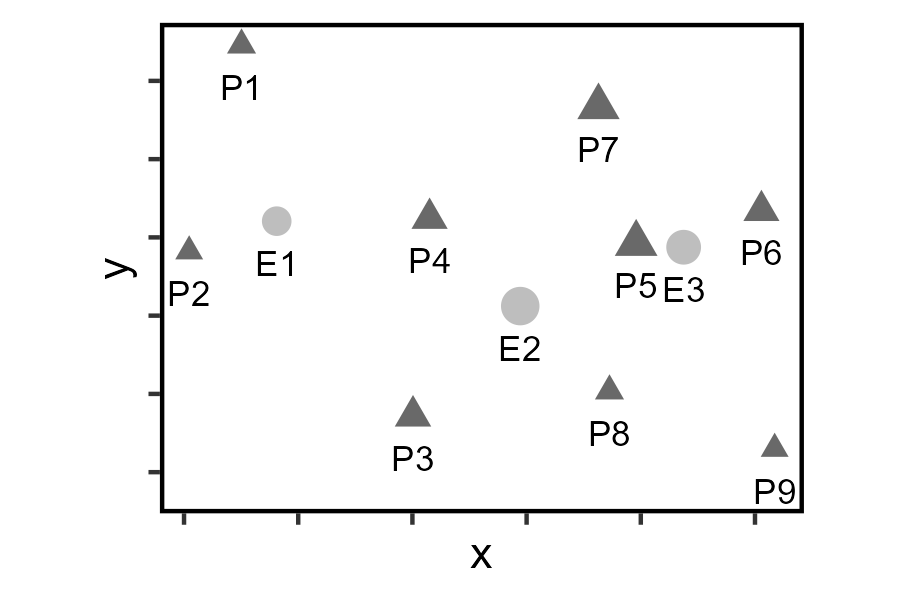
\includegraphics{images/figure-1.png}}\\
\bottomrule
\end{tabular}
\end{table}

\begin{figure}
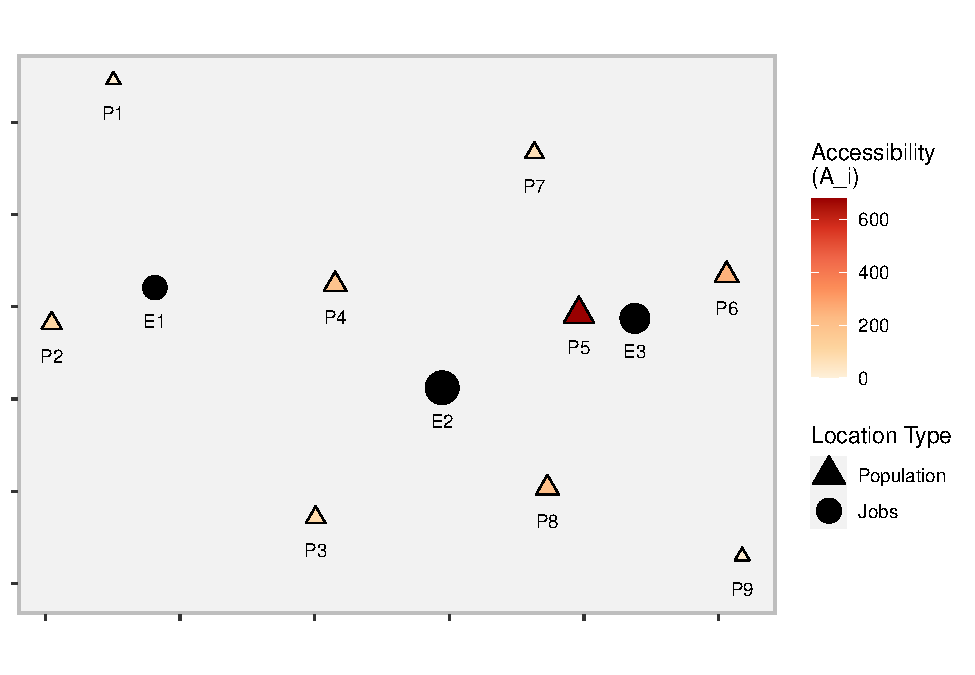
\includegraphics[width=1\linewidth]{Spatial-Availability_files/figure-latex/toy-example-accessibility-plot-1} \caption{\label{fig:toy-example-accessibility}Accessibility of jobs from population centers for the simple toy data set}\label{fig:toy-example-accessibility-plot}
\end{figure}

Figure \ref{fig:toy-example-accessibility} depicts three employment
centers locations (black circles), where the size of the symbol is in
proportion to the number of jobs at each location. We also see nine
population centers (triangles), where the size of the symbol is
proportional to the accessibility (\(A_i\)) to jobs. The accessibility
values illustrates the following:

\begin{itemize}
\item
  Population centers (triangles) in the middle of the plot are
  relatively close to all three employment centers and thus have the
  highest levels of job accessibility. Population center P5 is
  relatively central and close to all employment centers, and it is the
  closest population to the second largest employment center in the
  region. Unsurprisingly, this population center has the highest
  accessibility 680.64);
\item
  Population centers (triangles) near the left edge of the map (only in
  proximity to the small employment center) have the lowest levels of
  job accessibility. Population center P1 is quite peripheral and the
  closest employment center is also the smallest one. Consequently, it
  has the lowest accessibility with \(A_i=\) 17.12);
\end{itemize}

\hypertarget{issues-with-the-conventional-accessibility-measure}{%
\subsubsection{Issues With the Conventional Accessibility
Measure}\label{issues-with-the-conventional-accessibility-measure}}

Accessibility measures are excellent indicators of the intersection
between urban structure and transportation infrastructure . However,
beyond enabling comparisons of relative values they are not highly
interpretable on their own. For instance, from Figure
\ref{fig:toy-example-accessibility}, P1 has lower accessibility than P5
but despite the accessibility value for P1 being relatively low it is
still better than \emph{zero}. To address this interpretability issue,
previous research index and normalize values on a per-capita basis .
However, as recent critical research on accessibility discusses (see for
instance Paez, Higgins, Vivona (2019) and Allen and Farber (2019)),
these steps do not address the bias introduced through the uneven
multiple-counting of opportunities which are unconstrainted by
demand-side competition. We call this issue the `conglomeration effect'
and it arises as a result of the underlying mathematical assumption that
for conventional accessibility \(A_i\) all opportunities for all origins
\(i=1,\cdots,n\) are divisible and non-competitive. This results in
every opportunity entering the weighted sum once for every origin \(i\)
that can reach it. Put another way, if a densely populated population
center pops up next to P5 this center too will have a high accessibility
score since \(A_i\) does not consider competition of opportunities from
neighbouring demand centers. This neglect to constraint opportunity
counts (i.e., single-constraint) obscures the interpretability of
accessibility which may manifests in the following two ways of biased
estimation:

\begin{enumerate}
\def\labelenumi{\arabic{enumi})}
\item
  Demand centers in the less dense outer limits of the urban core may be
  assigned disproportionately \emph{high} accessibility values. These
  periphery areas are traditionally located in proximity to more dense
  urban demand centers and large urban opportunity centers and thus may
  have low travel cost to these large opportunity centers. Accessibility
  \(A_i\) does not consider opportunity-constraints and as such these
  periphery demand centers benefit from the high accessibility to
  opportunities without competition considerations from their more dense
  and more centrally located neighbours.
\item
  remote/isolated areas which are still within the region of the
  analysis and have regionally-relative low demand centers, opportunity
  centers, and travel cost to opportunity centers, are assigned
  disproportionately \emph{low} accessibility values. These
  remote/isolated areas may be sufficiently supplied with opportunities
  proportionate to their demand but is obscured by the artificially high
  accessibility awarded to periphery/other areas in which conglomeration
  disproportionately occurs.
\end{enumerate}

The spatially uneven multiple-counting of opportunities (i.e., the
conglomeration effect) leave decision makers unclear on how to interpret
resulting access values and all recent accessibility measures which seek
to improve interpretability are either vulnerable to this impact or
require potentially unrealistic assumptions . For instance, the floating
catchment areas (FCA) method increases interpretability by purporting to
account for competition, however, as discussed by Paez, Higgins, and
Vivona (2019), FCA methods are vulnerable to conglomeration effect. On
this same note, the doubly-constrained gravity model proposed by Allen
and Farber (2019) which is based on the FCA method accounts for
competition but requires that the magnitude of demand matches the
opportunities. As already mentioned, this assumption is not always
realistic for many opportunity types such as in the case of job seekers
and jobs.

To address the conglomeration effect and introduce a more realistic
assumption for opportunities, we propose a singly-constrained gravity
measure called \textbf{spatial availability}. This measure fundamentally
seeks to answer for a individual at a specific population center the
following questions: \emph{``many jobs are accessible, but the same jobs
are also accessible to my (possibly) numerous neighborus\ldots{} what
does a high accessibility actually mean to me?''} and \emph{``few jobs
are accessible but I am located in a remote area with proportionally few
neighbours\ldots{} what does low accessibility mean to me?''}.

\hypertarget{the-analytical-framework-of-spatial-availability}{%
\subsection{The Analytical Framework of Spatial
Availability}\label{the-analytical-framework-of-spatial-availability}}

Spatial availability \(V_{ij}\) is defined by opportunities \(O\) which
are proportionally allocated based on the relative population allocation
factor \(F^p_{ij}\) and cost of travel allocation factor \(F^c_{ij}\)
for all origins \(i\) to all destinations \(j\) as detailed in
(\ref{eq:spatial-availability}). In line with the gravity tradition, the
proposed framework distinguishes between opportunities at a destination
and demand for opportunities at the origin.

\begin{equation}
\label{eq:spatial-availability}
V_{ij} = O_j\frac{F^p_{ij} \cdot F^c_{ij}}{\sum_{i=1}^K F^p_{ij} \cdot F^c_{ij}}
\end{equation}

\noindent where:

\begin{itemize}
\tightlist
\item
  \(V_{ij}\) is spatial availability.
\item
  \(i\) is a set of origin locations in the region \(K\).
\item
  \(j\) is a set of destination locations in the region \(K\).
\item
  \(O_j\) is the number of opportunities at location \(j\) in the region
  \(K\).
\item
  \(F^p_{ij}\) is the proportional allocation factor of the population
  in \(i\) relative to the population in region \(K\).
\item
  \(F^c_{ij}\) is the proportion allocation factor of travel cost for
  \(i\) relative to the travel cost in region \(K\); it is a product of
  a monotonically decreasing (i.e., impedance) function associated with
  the cost of travel between \(i\) and \(j\).
\end{itemize}

To explain the analytical framework, the calculation of \emph{job
access} is illustrated with a simple step-by-step example for two
population centers (\(P_2\) and \(P_3\)) in the role of demand (i.e.,
the number of individuals in the labour market who ``demand''
employment) and one employment center (\(O_1\)) in the role of
opportunities.

Additionally, since spatial availability \(V_{ij}\) consists of these
two allocation factors, we detail first how the role of population
allocation factor \(F^p_{ij}\) in producing \(V^p_{ij}\), next the role
of the travel cost allocation factor \(F^c_{ij}\) in producing
\(V^c_{ij}\), and finally how both allocation factors in the final
general form of spatial availability \(V_{ij}\) are combined.

\hypertarget{population-and-travel-cost-allocation-factors}{%
\subsubsection{Population and Travel Cost Allocation
Factors}\label{population-and-travel-cost-allocation-factors}}

We begin with allocation based on demand; consider an employment center
\(j\) with \(O_j^r\) jobs of type \(r\). In the general case where there
are \(K\) population centers in the region, the following factor can be
defined (\ref{eq:pop-alloc-factor}).

\begin{equation}
\label{eq:pop-alloc-factor}
F^p_{ij} = \frac{P_{i\in r}^\alpha}{\sum_{i=1}^K P_{i\in r}^\alpha}
\end{equation}

The population allocation factor \(F^p_{ij}\) corresponds to the
proportion of the population in origin \(i\) relative to the rest of the
region's population centres \(K\). On the right hand side of the
equation, the numerator \(P_{i\in r}\) is the population at origin \(i\)
that is eligible and `demand' jobs of type \(r\) (maybe those with a
certain level of training or in a designated age group). The summation
in the denominator is over \(i=1,\cdots,K\), the number of population at
all origins \(i\) in the region \(K\). To modulate the effect of the
size in from this factor we also add an empirical parameter \(\alpha\)
(i.e., \(\alpha <1\) places greater weight on smaller centres relative
to larger ones while \(\alpha>1\) achieves the opposite effect). This
population allocation factor \(F^p_{ij}\) can now be used to
proportionally allocate a share of the jobs at a destination \(j\) to
all origin pairs.

More broadly, since the factor \(F^p_{ij}\) is a proportion, when it is
summed over \(i=1,\cdots,K\) it always equals to 1 (i.e.,
\(\sum_i^{K} F^p_{ij} = 1\)). This is notable since the share of jobs
(the spatial availability based on population \(V^p_{ij}\)) at each
destination \(j\) allocated to (i.e., available to) each origin is equal
to \(V^p_{ij} = O_j \cdot F^p_{ij}\) and since the sum of F\^{}p\_\{ij\}
is equal to 1 it follows that \(\sum_{i=1}^I V_{ij} = O_j\). In other
words, the number of jobs across the region is preserved. The result is
a proportional allocation of jobs (opportunities) to origins based on
population demand; this factor does not consider travel cost, that is
defined in the travel cost allocation factor \(F^c_{ij}\) which is
introduced shortly.

To illustrate the population allocation factor, consider an employment
center has 300 jobs (\(O_1= 300\)) in a region with two population
centers which have 240 and 120 people, respectively, (\(P_2= 240\) and
\(P_3 = 120\)). For simplicity, assume that all the population in the
region is eligible for these jobs, that is, that the entirety of the
population is included in the set \(r\). Also assume that \(\alpha=1\)
meaning the only impact on value is the population size for each center.
The population allocation factors \(F^p_{ij}\) for the jobs at \(O_1\)
for each population center \(P_2\) and \(P_3\) would be defined as
(\ref{eq:pop-alloc-factor-2populations}).

\begin{equation}
\label{eq:pop-alloc-factor-2populations}
\begin{array}{l}\
F^p_{2,1} = \frac{P_2 ^\alpha}{P_2^\alpha + P_3^\alpha} = \frac{240}{240 + 120} = \frac{240}{360}\\
F^p_{3,1} = \frac{P_3^\alpha}{P_2^\alpha + P_3^\alpha}  = \frac{120}{240 + 120} = \frac{120}{360}\\
\end{array}
\end{equation}

The \(F^p_{ij}\) values can be used to find a \emph{partial} spatial
availability of jobs which is only defined by the relative population
demanding jobs; this partial spatial availability \(V^p_{ij}\) for each
population center would be calculated as follows in
(\ref{eq:pop-alloc-factor-SA-2populations}).

\begin{equation}
\label{eq:pop-alloc-factor-SA-2populations}
\begin{array}{l}\
V^p_{2,1} = O_1 \cdot F^p_{2,1} = 300 \cdot \frac{240}{360} = 200 \\
V^p_{3,1} = O_1 \cdot F^p_{3,1} = 300 \cdot \frac{120}{360} = 100 \\
\end{array}
\end{equation}

It can be seen that when using only the proportional allocation factor
\(F^p_{ij}\) to calculate spatial availability (differentiated here by
being defined as \(V^p_{ij}\) instead of \(V_{ij}\)), proportionally
more jobs are allocated to the bigger population center (i.e., 2 times
more jobs as it is 2 times larger in population). We can also see that
the sum of spatial availability for all population centers is equal to
the sum of jobs, i.e., total opportunities are preserved. However, as
mentioned, using only the proportional allocation factor \(F^p_{ij}\) to
calculate spatial availability does not account for how far population
centers \(P_2\) or \(P_3\) are from employment center \(O_1\). To
account for this effect we introduce a second allocation factor
\(F^c_{ij}\) based on distance to the employment centers defined in
(\ref{eq:tcost-alloc-factor}).

\begin{equation}
\label{eq:tcost-alloc-factor}
F^c_{ij} = \frac{f(c_{ij})}{\sum_{i=1}^K f(c_{ij})}\\
\end{equation}

Where \(c_{ij}\) is the cost (e.g., the distance, travel time, etc.)
from population center \(i\) to employment center \(j\), and
\(f(\cdot)\) is an impedance function that is a monotonically decreasing
function of cost (\(c_{ij}\)); in other words, the travel cost
allocation factor \(F^c_{ij}\) serves to proportionally allocates more
jobs to closer locations through an impedance function. To continue
illustrating, assume that the impedance function is a negative
exponential function and assume that \(\beta\) (which modulates the
steepness of the impedance effect and is an empirical parameter) is the
value of 1 for simplicity. Also suppose that the distance from
population center \(P_2\) to employment center \(O_1\) is 0.6 km, and
the distance from population center \(P_3\) to employment center \(O_1\)
is 0.3 km. The proportional allocation factor \(F^p_{ij}\) for the jobs
at \(O_1\) for both population centers \(P_2\) and \(P_3\) is defined as
follows (\ref{eq:tcost-allocation-factor-2populations}).

\begin{equation}
\label{eq:tcost-allocation-factor-2populations}
\begin{array}{l}\
F^c_{2,1} = \frac{\exp(-\beta \cdot D_{2,1})}{\exp(-\beta \cdot D_{2,1}) + \exp(-\beta \cdot D_{3,1})} = \frac{\exp(-0.6)}{\exp(-0.6) + \exp(-0.3)} = 0.426\\
F^c_{3,1} = \frac{\exp(-\beta \cdot D_{3,1})}{\exp(-\beta \cdot D_{2,1}) + \exp(-\beta \cdot D_{3,1})}  = \frac{\exp(-0.3)}{\exp(-0.6) + \exp(-0.3)} = 0.574\\
\end{array}
\end{equation}

We can see that the proportional allocation factor for \(P_3\) is larger
than \(P_2\) since the distance to \(O_1\) is shorter. Using the travel
cost proportional allocation factors \(F^c_{ij}\) as defined in
(\ref{eq:tcost-allocation-factor-2populations}), we can now calculate
the spatial availability of jobs for each population center based only
on \(F^c_{ij}\) and the jobs available \(O_1\) to these two competing
population centers (note: \(V^c_{ij}\) not the complete \(V_{ij}\)) as
follows in (\ref{eq:tcost-allocation-factor-SA-2populations}).

\begin{equation}
\label{eq:tcost-allocation-factor-SA-2populations}
\begin{array}{l}\
V^c_{2,1} = O_1 \cdot F^c_{2,1} = 300 \times 0.426 = 127.8\\
V^c_{3,1} = O_1 \cdot F^c_{3,1} = 300 \times  0.574 = 172.2\\
\end{array}
\end{equation}

As shown, the spatial availability defined by \(F^c_{ij}\) (i.e.,
\(V^c_{ij}\)) allocates \(P_3\) a larger share of jobs since the
population center is closer to \(O_1\). However, as previously
discussed, \(P_3\) has a smaller population than \(P_2\), so \(P_2\)
receives a larger share of jobs when spatial availability when it is
defined by \(F^p_{ij}\) (i.e., \(V^p_{ij}\)). It is necessary to combine
both population and travel cost factors to accurate reflect demand;
these two components are in line with how demand is conventionally
modelled in accessibility calculations. Fortunately, since both
\(F^c_{ij}\) and \(F^p_{ij}\) preserve the total number of opportunities
(jobs) as they independently sum to 1, they can be combined
multiplicatively to calculate the proposed spatial availability
(\(V_{ij}\)) which considers demand to be based on both population and
travel cost.

\hypertarget{putting-spatial-availability-together}{%
\subsubsection{Putting Spatial Availability
Together}\label{putting-spatial-availability-together}}

We can combine the proportional allocation factors by population
\(F^p_{ij}\) and travel cost \(F^c_{ij}\) and calculate spatial
availability \(V_{ij}\) as introduced in (\ref{eq:spatial-availability})
and repeated below:

\[
V_{ij} = O_j\frac{F^p_{ij} \cdot F^c_{ij}}{\sum_{i=1}^K F^p_{ij} \cdot F^c_{ij}}
\]

To complete the illustrative example of employment center \(O_1\) and
population centers \(P_2\) and \(P_3\), the resulting spatial
availability \(V_{ij}\) is calculated for both population centers is
calculated in (\ref{eq:SA-2populations}).

\begin{equation}
\label{eq:SA-2populations}
\begin{array}{l}\
V_{2,1} = O_1\cdot \frac{F^p_{2,1} \cdot F^c_{2,1}}{F^p_{2,1} \cdot F^c_{2,1} + F^p_{3,1} \cdot F^c_{3,1}} = 300 \frac{\big(\frac{2}{3} \big) \big(0.426 \big)}{\big(\frac{2}{3} \big) \big(0.426 \big) + \big(\frac{1}{3} \big) \big(0.574 \big)} = 179.4\\
V_{3,1} = O_1\cdot \frac{F^p_{3,1} \cdot F^c_{3,1}}{F^p_{2,1} \cdot F^c_{2,1} + F^p_{ik} \cdot F^c_{ik}} = 300 \frac{\big(\frac{1}{3} \big) \big(0.574 \big)}{\big(\frac{2}{3} \big) \big(0.426 \big) + \big(\frac{1}{3} \big) \big(0.574 \big)}  =  120.6 \\
\end{array}
\end{equation}

As can be seen, fewer number of jobs are allocated to population center
\(P_2\) compared to the allocation by population only, to account for
the higher cost of reaching the employment center. On the other hand,
distance alone allocated more jobs to the closest population center
(i.e., \(P_3\)), but since it is smaller, it also gets a smaller share
of the jobs overall. To reiterate, the sum of jobs at employment center
\(O_1\) that are allocated to population centers \(P_2\) and \(P_3\)
simultaneously based on \emph{population-} and \emph{travel cost}
allocation factors are preserved (i.e., \(V_{2,1} + V_{3,1} = O_1\)).

In the common case that population centers have multiple destination
opportunities \(j\), availability is simply the sum of
(\ref{eq:spatial-availability}) for all opportunities \(J\) (i.e.,
\(V_i = \sum_{j=1}^J V_{ij}\)). This quantity represents opportunities
(e.g., jobs) that can be accessed from \(i\) and that are \emph{not}
allocated to a competitor: therefore the weighted sum of available
opportunities. Compare \(V_i\) to the singly-constrained gravity model
(see Wilson (1971)) . In essence, \(V_i\) is the result of constraining
\(A_i\) to match one of the marginals in the origin-destination table,
the known total of opportunities.

Since the sum of opportunities is preserved in the procedures above, it
is possible to calculate a highly interpretable measure of spatial
availability per capita (lower-case \(v_i\)) as follows in
(\ref{eq:SA-per-capita}).

\begin{equation}
\label{eq:SA-per-capita}
v_i = \frac{V_i}{P_i}
\end{equation}

To complete the illustrative example, the per capita spatial
availability of jobs would be calculated as follows in
(\ref{eq:SA-per-capita-2populations}).

\begin{equation}
\label{eq:SA-per-capita-2populations}
\begin{array}{l}\
v_{2,1} = \frac{V_{2,1}}{P_2} =  \frac{179.4}{240} = 0.8\\
v_{3,1} =  \frac{V_{3,1}}{P_3} =  \frac{120.6}{120} = 1.0\\
\end{array}
\end{equation}

We can see that since \(P_3\) is closer to \(O_1\) and has less
competition (as it has a smaller population than \(P_2\)), \(P_3\)
benefits with a higher spatial availability of jobs per capita.

Where the overall ratio of jobs to population in the region is
\(300/(240 + 120)=\) 0.83, the spatially available jobs per capita at
\(k\) is closer to unity.

\hypertarget{empirical-example-spatial-availability-and-accessibility-of-jobs-in-the-ggh}{%
\section{Empirical Example: Spatial Availability and Accessibility of
Jobs in the
GGH}\label{empirical-example-spatial-availability-and-accessibility-of-jobs-in-the-ggh}}

In this section, we use two empirical examples to demonstrate how the
spatially uneven multiple-counting of opportunities (i.e.,
conglomeration effect) inherent to the accessibility measure
(\ref{eq:conventional-accessibility}) introduces spatial bias and
obscures interpretability. This conglomeration effect is highlighted by
calculating spatial availability (\ref{eq:spatial-availability}) and
comparing the relative difference between the two measures. The first
example demonstrates how accessibility broadly overestimates \emph{job
access} (relative to spatial availability) and particularly
overestimates job access for areas in the less dense outer limits of the
urban core. The second example demonstrates how accessibility
underestimates job access for areas in the urban periphery. Both
examples are based on the same empirical data set for home-based work
trips in the Greater Golden Horseshoe (GGH) area. We first introduce the
data used, then calibrate the impedance function, and finally illustrate
the two examples.

\hypertarget{data}{%
\subsection{Data}\label{data}}

The 2016 Transportation Tomorrow Survey (TTS) data for 20 municipalities
contained within the GGH area in the province of Ontario, Canada (43.6°N
79.73°W) is used within this section (Figure
\ref{fig:TTS-16-survey-area}). This data set includes home-based origins
and employment destinations defined by centroids of Traffic Analysis
Zones (TAZ) (n=3764), the number of jobs (n=3081900) and workers
(n=3446957) at each origin and destination, and the trips from origin to
destination for the morning home-to-work commute (n=3446957).

Also included are travel times and cost of travel from origin to
destination by car; travel times are calculated using the R package
\texttt{r5r} (Rafael H. M. Pereira et al., 2021) and an impedance
function based on these travel times is derived. It is important to note
that for simplicity, all trips within this data set are assumed to be
taken by car, and the travel time is calculated from an origin TAZ
centroid to a destination TAZ centroid. The centroid is snapped to the
nearest street line by \texttt{r5r} and the travel time is calculated
for all trips assuming a car travel mode and a department of 7:00am on
Wednesday October 2021, an arbitrary date selected by the authors.
Additionally, only travel times less than or equal to 180 mins (3 hrs);
this threshold represents 99\% of trip's travel times which are
summarized in the descriptive statistics in Table
\ref{tab:TTS-16-desc-stats}. All data and data preparation steps can be
freely explored in companion R data-package
\href{https://github.com/soukhova/AccessPack}{\texttt{AccessPack}}.

\begin{figure}

{\centering 
\includegraphics[width=0.7\linewidth]{images/Greater-Golden-Horseshoe-Map} 

}

\caption{\label{fig:TTS-16-survey-area}The TTS 2016 study area within the Greater Golden Horseshoe in Ontario, Canada.}\label{fig:TTS-16-survey-area}
\end{figure}

\begin{table}

\caption{\label{tab:unnamed-chunk-1}\label{tab:TTS-16-desc-stats}Descriptive statistics of the TTS 2016 dataset for the Greater Golden Horshoe Area}
\centering
\begin{tabular}[t]{l|l|l}
\hline
  & Trips & Travel\_Time\\
\hline
 & Min.   :   1.00 & Min.   :  0.00\\
\hline
 & 1st Qu.:  14.00 & 1st Qu.: 13.00\\
\hline
 & Median :  22.00 & Median : 20.00\\
\hline
 & Mean   :  33.44 & Mean   : 23.39\\
\hline
 & 3rd Qu.:  38.00 & 3rd Qu.: 30.00\\
\hline
 & Max.   :1129.00 & Max.   :179.00\\
\hline
 & NA & NA's   :3507\\
\hline
\end{tabular}
\end{table}

\hypertarget{calibrating-an-impedance-function}{%
\subsection{Calibrating an Impedance
Function}\label{calibrating-an-impedance-function}}

In the toy data set introduced in the
\protect\hypertarget{accessibility-numerical-example}{}{Numerical
Accessibility Example} section, an arbitrary negative exponential
function describing travel cost (as a function of distance) was used as
the impedance function to derive both accessibility and spatial
availability. In this empirical data set, since the travel time is
calculated based on the existing street network in the GGH, an empirical
trip length distribution (TLD) is defined and used to derive an
impedance function. For background, a TLD is the representation of the
likelihood that a proportion of trips are taken at a specific travel
cost and are widely used to derive impedance functions in accessibility
research .

The empirical TLD for this data set is represented by black data points
in Figure \ref{fig:TLD-Gamma-plot}). As can be observed, this empirical
distribution appears to follow a gamma distribution, as such, this
theoretical distribution along with other common TLD distributions such
as log-normal and exponential distributions were fitted to the empirical
TLD. The maximum likelihood estimation method and Nelder-Mead method for
direct optimization available within the \texttt{fitdistrplus} package
(Delignette-Muller and Dutang, 2015) was used . Based on goodness-of-fit
criteria and diagnostics presented in Appendix Figure
\ref{fig:impedance-function-plot} and \ref{fig:plot-cullen-frey}, the
gamma distribution was selected and is represented as a red line in
Figure \ref{fig:TLD-Gamma-plot}.

\begin{figure}
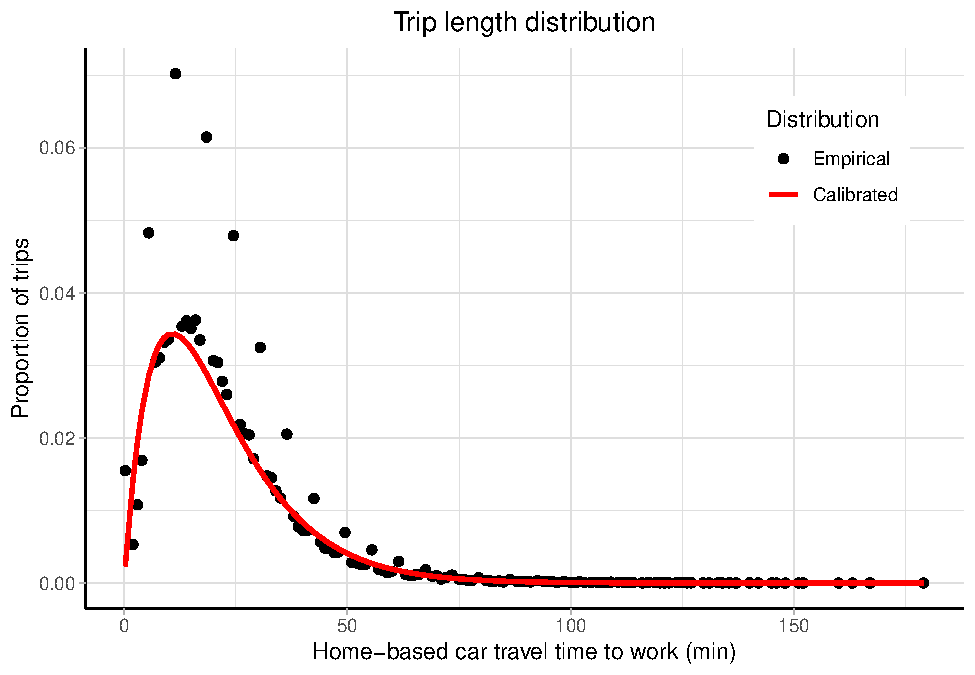
\includegraphics[width=1\linewidth]{Spatial-Availability_files/figure-latex/TLD-Gamma-plot-1} \caption{\label{fig:TLD-Gamma-plot}Empirical TTS 2016 home-based car trip length distribution (black) and calibrated gamma distribution impedance function (red)}\label{fig:TLD-Gamma-plot}
\end{figure}

The resulting calibrated gamma distribution, which serves as the
impedance function for the empirical data set, is given in the following
general form where the estimated `shape' is \(\alpha\), the estimated
`rate' is \(\beta\), and \(\Gamma(\alpha)\) is defined in
(\ref{gamma-dist}). The calculated shape and rate parameter is 2.019 and
0.094 respectively. We would like to reiterate that this impedance
function, though it is derived using empirical data, assumes all
home-to-work trips in the 2016 TTS data set are all taken by car. In
reality there is a modal split but for illustrative purposes, the same
impedance function is used to calculate accessibility and spatial
availability in the following examples.

\begin{equation}
\label{gamma-dist}
\begin{array}{l}\ 
f(x, \alpha, \beta) = \frac {x^{\alpha-1}e^{-\frac{x}{\beta}}}{ \beta^{\alpha}\Gamma(\alpha)} \quad \text{for } 0 \leq x \leq \infty\\

\Gamma(\alpha) =  \int_{0}^{\infty} x^{\alpha-1}e^{-x} \,dx\\
\end{array}
\end{equation}

\hypertarget{access-to-jobs-in-toronto}{%
\subsection{Access to jobs in Toronto}\label{access-to-jobs-in-toronto}}

Toronto is the largest city in the GGH and represents a significant
subset of workers and jobs in the GGH; 50\% of workers in the GGH travel
to jobs in Toronto and 72\% of jobs are located within Toronto. As later
discussed, this significant subset of jobs illustrates the first issue
associated with the accessibility measure conglomeration effect :
neglecting to include the single-constraint overestimates job access for
TAZ with a low proportion of workers that are next to TAZ with a high
proportion of jobs and workers.

Accessibility is first calculated and presented in Figure
\ref{fig:plot-access-SA-Toronto-TTS}. The higher the accessibility
value, the more accessible places of employment are to home-based
origins. It can be briefly summarized that the accessibility values
follow a radial trend where the majority of TAZs in Toronto have high
accessibility values and values decrease in TAZs which are further from
the city boundary. This finding is echoed in many studies and indicates
that the closer one lives to Toronto, the more opportunities for
employment they will have access to.

Next, job access is calculated using the spatial availability measure
and is present alongside the accessibility plot in Figure
\ref{fig:plot-access-SA-Toronto-TTS}. Similar to the accessibility plot,
the higher the value the more the more access that TAZ has to jobs in
the city of Toronto. However, since spatial availability constraints the
total number of opportunities counted, high values of spatial
availability can be seen as higher access to \emph{available} jobs and
we can observe which TAZs have job access values which are above or
below the regional average of 638.

\begin{figure}
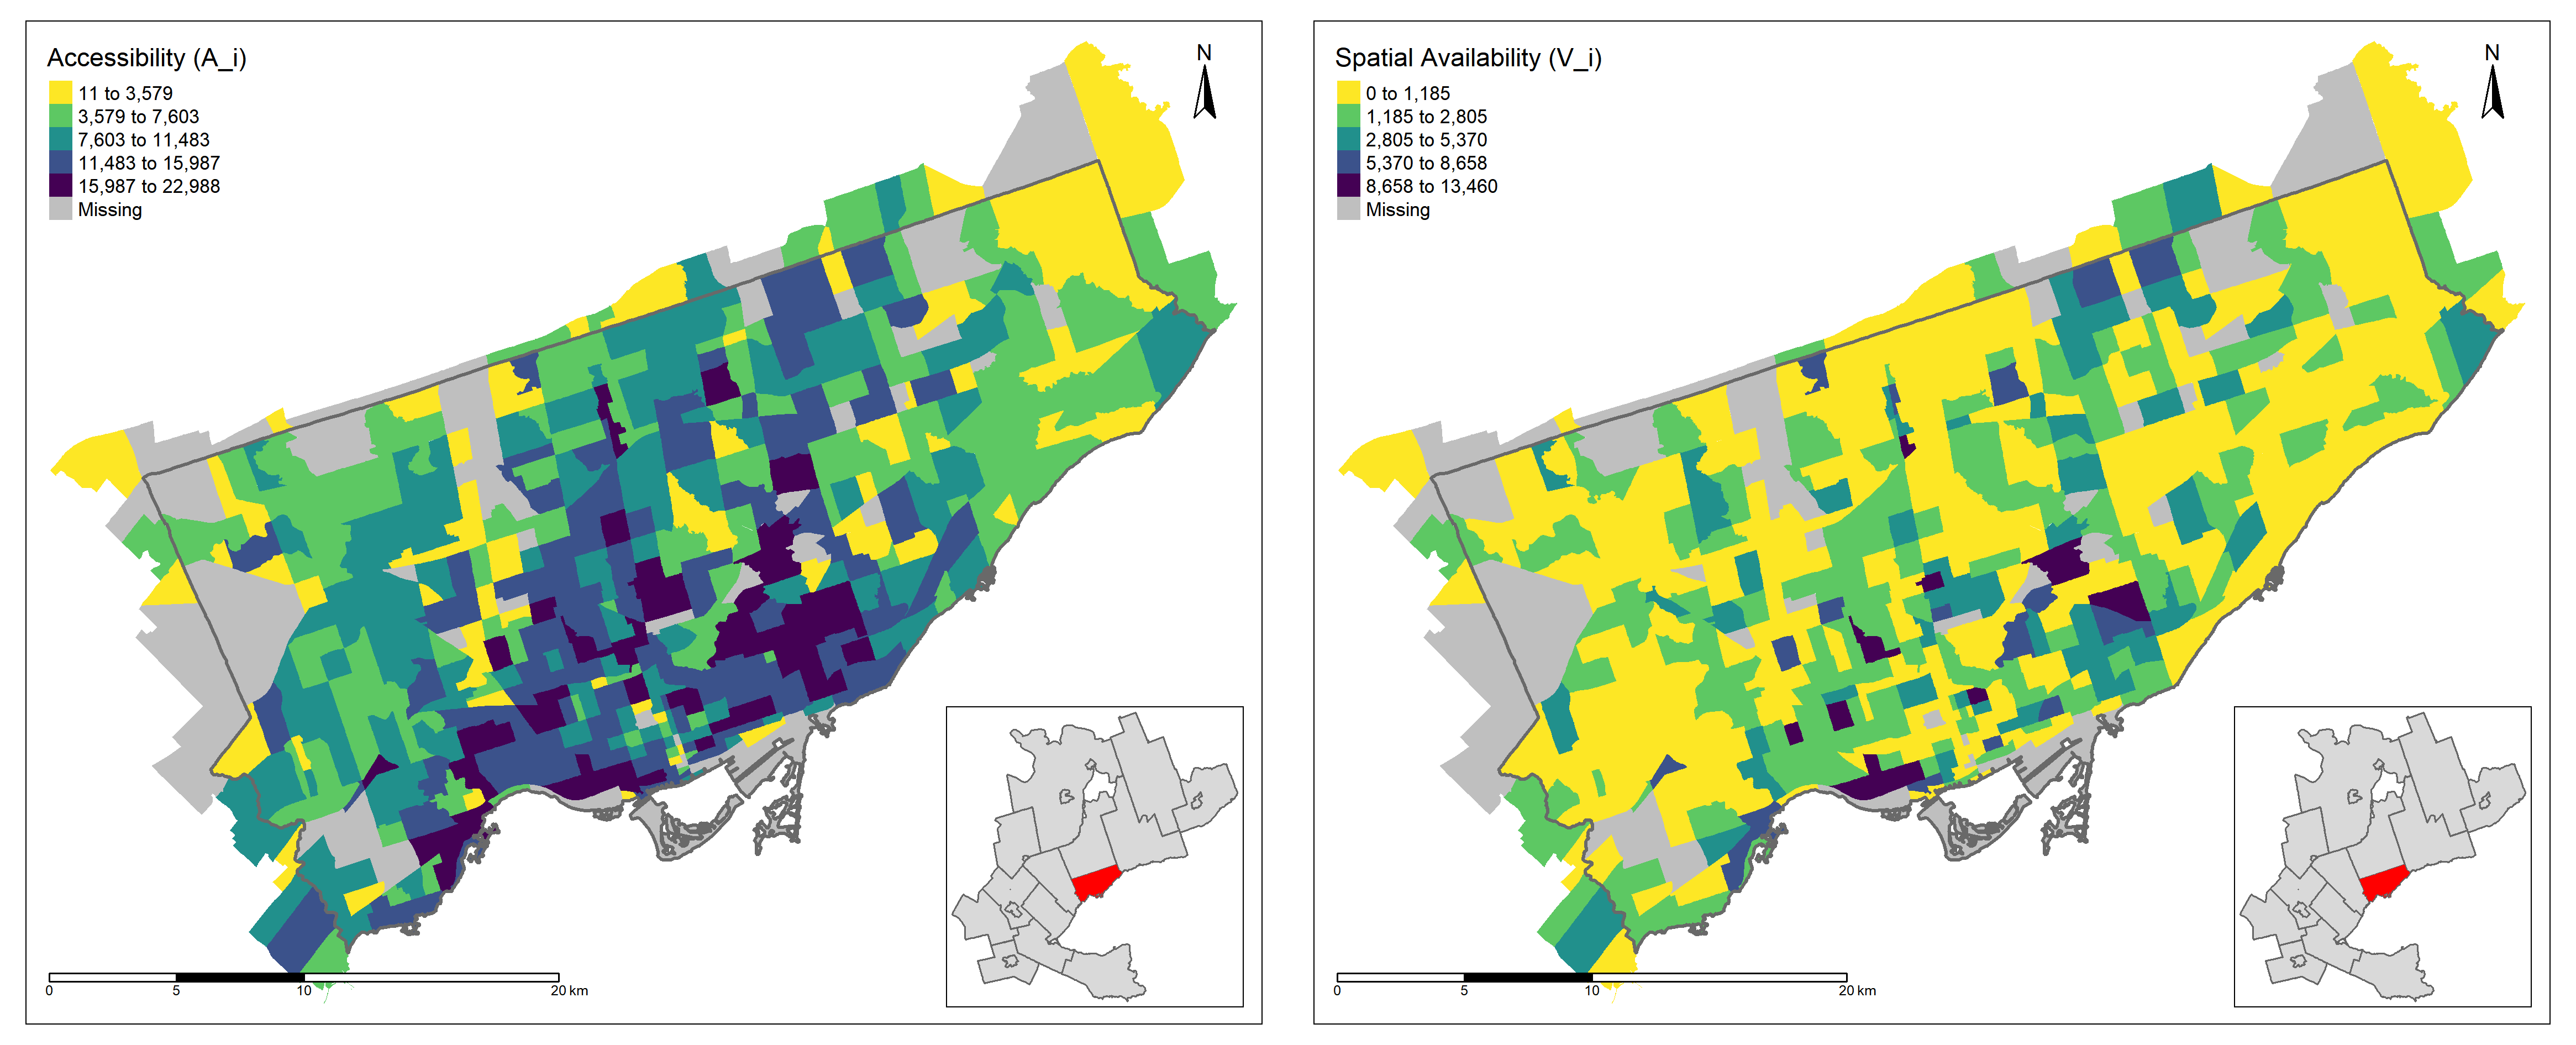
\includegraphics[width=1\linewidth]{Spatial-Availability_files/figure-latex/plot-access-SA-Toronto-TTS-1} \caption{\label{fig:plot-access-SA-Toronto-TTS}Calculated accessibility (top) and spatial availability (bottom) of employment from origins in the GGH to destinations in the City of Toronto.}\label{fig:plot-access-SA-Toronto-TTS}
\end{figure}

\newpage

The visual differences between accessibility and spatial availability
plots in Figure \ref{fig:plot-access-SA-Toronto-TTS} are stark. The TAZ
within and 10-20 km outside of Toronto's boundary have relatively lower
access values (i.e., fewer reds and oranges) as measured by spatial
availability than as measured by accessibility. There are also more
pockets of low job access (i.e., blues) within the city of Toronto when
measured by spatial availability; this observation is in line with
empirical quantitative work describing the spatially uneven job
accessibility landscape in Toronto .

To enhance the interpretability of spatial availability, job access can
be normalized to provide more meaningful insight on how many jobs are
\emph{available} on average for each TAZ. This normalization, shown in
Figure \ref{fig:plot-avail-Toronto-TTS-per-worker}, demonstrates which
TAZ have above (reds) and below (blue) the average (0.38) available jobs
per worker in the GGH to jobs located within the city of Toronto.
Overall, similar to the non-normalized spatial availability measure,
this figure demonstrates that job access is lower within and around
Toronto than the accessibility measure. We can also observe a similar
uneven spatial distribution of job access within Toronto (as also shown
in the spatial availability plot in Figure
\ref{fig:plot-access-SA-Toronto-TTS}) where job access is consistently
far about the average and often greater than 1 job per worker for the
soouth-central and south-west TAZ in Toronto, this trend is not as
pronounced in the south-east and other pockets in the City. This uneven
distribution of job access has been explained by some studies to be a
result of\ldots{} .

\begin{figure}
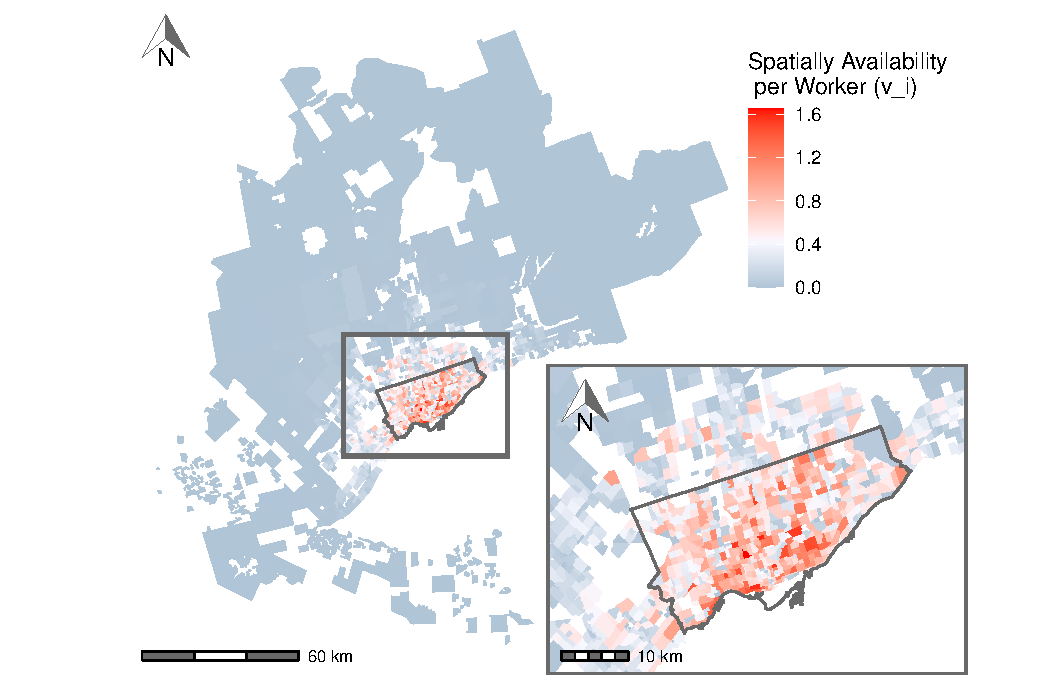
\includegraphics[width=1\linewidth]{Spatial-Availability_files/figure-latex/plot-avail-Toronto-TTS-per-worker-1} \caption{\label{fig:plot-avail-Toronto-TTS-per-worker}Calculated spatial availability of employment, per worker, from origins in the GGH to destinations in the City of Toronto.}\label{fig:plot-avail-Toronto-TTS-per-worker}
\end{figure}

\newpage

\hypertarget{access-to-jobs-in-the-ggh}{%
\subsection{Access to jobs in the GGH}\label{access-to-jobs-in-the-ggh}}

In this section we calculate job access for \emph{all} jobs in the GGH
for all origins in the GGH using both accessibility and spatial
availability measures. As will be later elaborated, the full TTS data
set demonstrates the second issue associated with the conglomeration
effect expressed by the accessibility measure. More specifically, this
issue underestimates job access for TAZ which are on located in the
periphery of the GGH and have relatively-low proportion of workers and
are relatively isolated (by travel cost) from the Toronto which has the
highest density of jobs. The first issue, namely the over estimation of
the TAZs which are on the outer limits outside the Toronto border can
also be observed.

Accessibility and spatial availability are both calculated and presented
in Figure \ref{fig:plot-access-SA-GGH-TTS}. Interestingly, despite the
majority of jobs being located within Toronto - general trends are
similar for both accessibility plots but not for both spatial
availability plots. For instance, the accessibility values follow a
radial trend where the majority of TAZs in Toronto have high
accessibility values and values decrease in TAZs which are further from
the city boundary. However, it can be seen that the radial effect is
less pronounced and TAZs outside of Toronto appear to have a higher
accessibility score. Conversely, spatial availability does not appear to
follow a radial trend as depicted in the previous plot in Figure
\ref{fig:plot-access-SA-Toronto-TTS}. Job access, as measured by spatial
availability, appears much more even throughout the GGH (in comparison
to job access as measured by accessibility). This can be noted in higher
values around the north east and south west periphery TAZs and more
moderate values in and around Toronto. This distribution of job access
in the GGH may be more realistic as qualitative and quantitative studies
have demonstrated that as operating costs continue to increase in
Toronto, more and different types of employment centers are operating in
the periphery of the GGH .

\begin{figure}
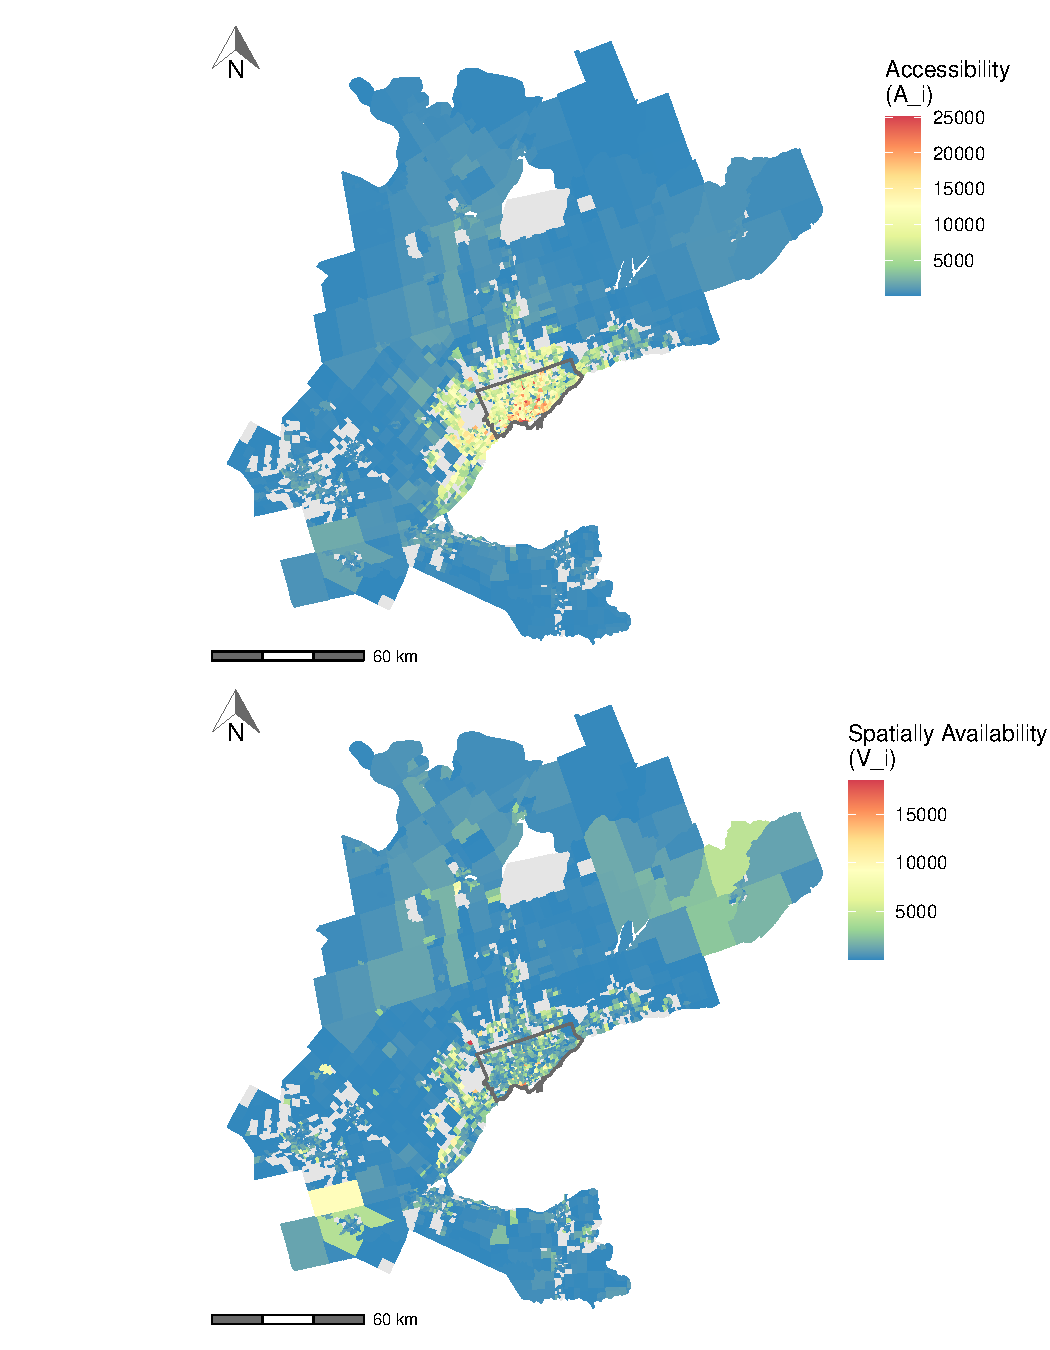
\includegraphics[width=1\linewidth]{Spatial-Availability_files/figure-latex/plot-access-SA-GGH-TTS-1} \caption{\label{fig:plot-access-SA-GGH-TTS}Calculated accessibility (top) and spatial availability (bottom) of employment from origins in the GGH to destinations in the GGH.}\label{fig:plot-access-SA-GGH-TTS}
\end{figure}

\newpage

Similar to the per capita spatial availability figure for jobs in the
Toronto (Figure \ref{fig:plot-avail-Toronto-TTS-per-worker}), Figure
\ref{fig:plot-avail-GGH-TTS-per-worker} depicts which TAZs have above
average, below average, and average (0.89) access to jobs per capita
considering all jobs and workers in the GGH. We can some similar general
trends, such as a higher concentration of jobs per capita are available
in TAZs which are within the city of Toronto. However, the plot is
distinct and more similar to the spatial availability plot for this data
set, where we can see the jobs per capita values are more evenly
distributed throughout the GGH, relative to the trends in the
accessibility plot. We can also see higher jobs per capita in employment
areas in different cites such as Mississauga and Burlington (south-west
of Toronto), Waterloo and Brantford (even more south-west of Toronto),
and Hamilton and Niagra (south of Toronto).

Again, spatial availability can also be represented on a per-worker
basis and a similar trend between spatial availability in Figure
\ref{fig:plot-avail-Toronto-TTS-per-worker} can be seen for all GGH jobs
in Figure \ref{fig:plot-avail-GGH-TTS-per-worker}. Interestingly, when
considering the jobs which are \emph{available}, many areas outside of
Toronto have similar jobs per capita values as TAZ in Toronto. This is
contrary to the common belief that Toronto is one of the only hubs for
employment opportunities . Urban centers in Brantford, Guelph, Missauga,
Burlington, and Niagra have TAZs which are far above the the average
jobs per capita and compare to TAZ within Toronto. This suggests that
these less densely populated areas may have sufficient employment
opportunities for their population and this finding is obscured when
only considering the accessibility measure for job access.

It is also worth noting that within the full sample of the GGH, there is
almost two times more jobs per capita than the rate for Toronto jobs per
GGH capita. This suggests that all GGH people who work in the city of
Toronto, on average, face more competition for jobs than all GGH people
who work anywhere in the GGH. The causes for this trend are numerous and
can include \ldots. as mentioned by study .

\begin{figure}
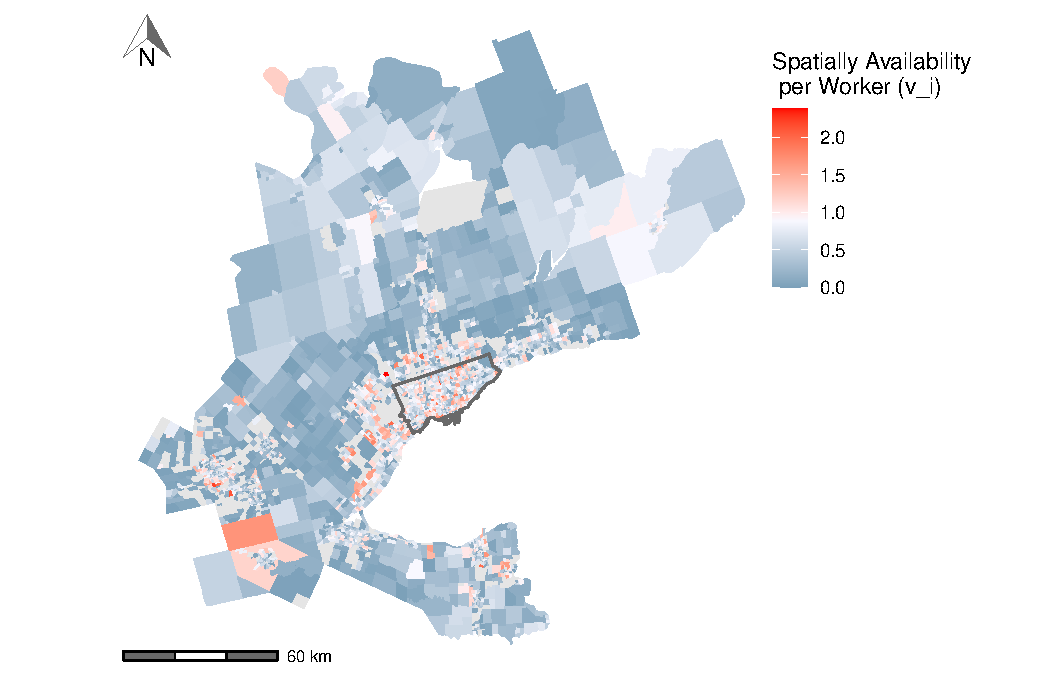
\includegraphics[width=1\linewidth]{Spatial-Availability_files/figure-latex/plot-avail-GGH-TTS-per-worker-1} \caption{\label{fig:plot-avail-GGH-TTS-per-worker}Calculated spatial availability of employment, per worker, from origins in the GGH to destinations in the City of Toronto.}\label{fig:plot-avail-GGH-TTS-per-worker}
\end{figure}
\newpage

\hypertarget{discussion}{%
\section{Discussion}\label{discussion}}

We have used both accessibility and spatial availability to measure
access to jobs and have visually compared trends for the empirical GGH
data set in the previous section. To build on these findings, a thorough
comparative discussion is detailed in this section in which we return to
the two issues produced by the conglomeration effect as associated with
the accessibility \(A_i\) measure. As we described, accessibility has
the tendency to overestimate job access for areas which may experience
high competition (issue 1) and underestimate job access for areas with
low competition (issue 2).

To compare both accessibility and spatial availability, we calculate
their relative magnitudes by re-scaling both measures from 0 to 100
where each value of the measure is divided by the maximum value as
described in Equation \ref{eq:index-measures} by \(A^I_{ij}\) and
\(V^I_{ij}\). This re-scaling process is done since accessibility cannot
be meaningfully compared through normalization on a per worker basis
since the methodology inherently multiple-counts opportunities which is
not the case for spatial availability. Re-scaling is repeated for both
measures for the subset of jobs in Toronto and for all jobs in the GGH
and differences are calculated as described in Equation
\ref{eq:dif-index-measures}.

\begin{equation}
\label{eq:index-measures}
\begin{array}{l}\
A^I_{ij} = \frac{A_{ij}}{\max(A_{ij})}\cdot100\\
V^I_{ij} = \frac{V_{ij}}{\max(V_{ij})}\cdot100\\
\end{array}
\end{equation}

\begin{equation}
\label{eq:dif-index-measures}
Dif_{ij} = \frac{V^I_{ij} - A^I_{ij}}{A^I_{ij}}\cdot100
\end{equation}

\hypertarget{overestimating-jobs-access-issue-1}{%
\subsection{Overestimating jobs access (issue
1)}\label{overestimating-jobs-access-issue-1}}

For the subset of jobs in Toronto and all origins in the GGH, 98.9\% of
TAZ have re-scaled spatial availability values whcih are lower than
re-scaled accessibility values. Of this 98.9\%, the spatial availability
value is on average -80.64\% different than the accessibility value and
the difference ranges between -2.95\% to -99.9\%. Furthermore, to
emphasis the similarity of this difference measure between neighbourhing
TAZs, the spatial autocorrelation is calculated using Moran's I
statistic (Anselin, 1995) and TAZ with a significant p-value
(\(p\le 0.10\)) are more vividly presented. Figure
\ref{fig:plot-local-i-Toronto} displays the described plotted
comparison, where the more negative the value, the more the
accessibility measure overestimation job access relative to spatial
availability for each TAZ. It should be noted that although the majority
of TAZ job access values are overestimated by accessibility, the 23 TAZ
which are underestimated are shown in grey.

\begin{figure}
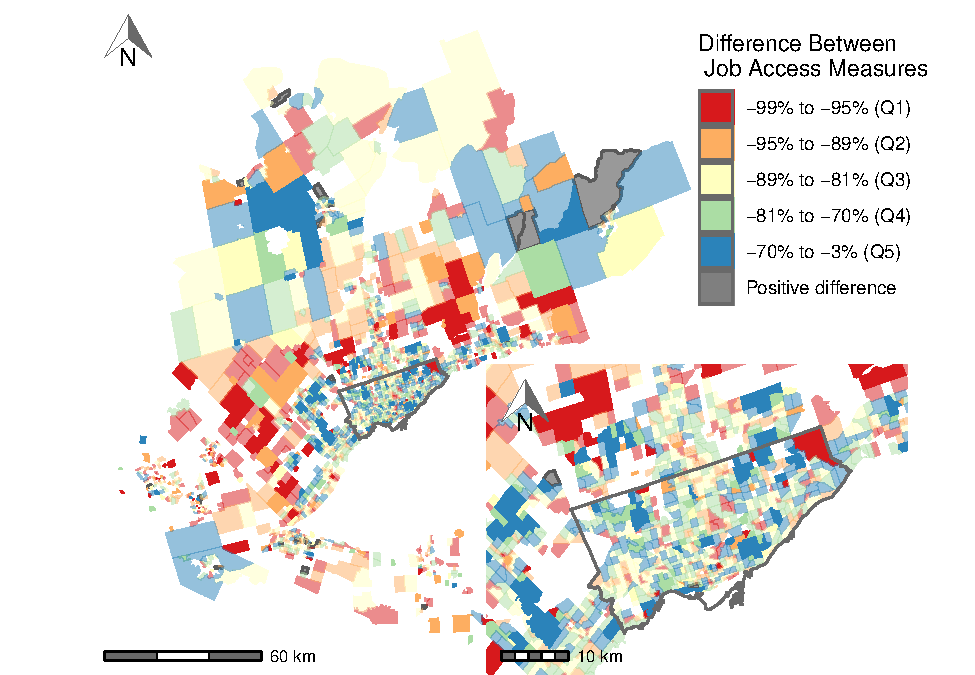
\includegraphics[width=1\linewidth]{Spatial-Availability_files/figure-latex/plot-local-i-Toronto-1} \caption{\label{fig:plot-local-i-Toronto}Difference between re-scaled the accessibility and the spatial availability job access measure in the context of employment from origins in the GGH to destinations in the City of Toronto. Values are expressed in five quantile ranges. Vivid TAZs represent a significant spatial autocorrelation and dimmed TAZs represent a non-signficant autocorrelation as measured by Local Moran's I. TAZs with values which are higher than re-scaled accessibility (positive difference) are shown fully in grey.}\label{fig:plot-local-i-Toronto}
\end{figure}

We can see from Figure \ref{fig:plot-local-i-Toronto} that when we
re-scale both job access values, accessibility consistently overestimate
job access compared to the spatial availability measure for jobs within
the city of Toronto and all people within the GGH who travel to Toronto
for work. Overestimation ranges from -100\% to -3\% and is on average
-81\%. However, while job access is consistently overestimated, it is
overestimated in a variable way. The TAZs with the largest difference in
measure are depicted in red and orange (quantiles 1 and 2) and can be
seen, in sometimes concentrated clusters (as indicated by the 2044 TAZs
with a significant Moran I's statistic) approximately 10-20 kms outside
of Toronto city border and along the south side of the GGH. These TAZs
also have a relatively low density of people who work in Toronto and as
such the difference between measures has a significant correlation (
0.877) with the number of workers in each TAZ.

Nonetheless, the density of workers within each TAZs alone does not
fully explain the variation in overestimation. The number of
opportunities and the travel cost also factors in the calculation of
both accessibility and spatial availability. From the perspective of
accessibility \(A_i\), job access does not consider
opportunity-constraints and as such the extensively overestimated TAZs
benefit from overestimated job access without any competition
considerations from their more dense and more centrally located
neighbours (within the city of Toronto) and their more peripherally
located but more relatively more worker-dense peripheral neighbours.
Spatial availability \(V_i\) considers this competition by
proportionally allocating jobs to these TAZs relative to their travel
cost and worker population. In other words, these overestimated TAZs
reflect the incident in which travel cost outpaced the number of workers
and thus the proportionately allocated opportunities are significantly
fewer when measured by spatial availability \(V_i\) instead of
accessibility \(A_i\).

\hypertarget{underestimating-jobs-access-issue-2}{%
\subsection{Underestimating jobs access (issue
2)}\label{underestimating-jobs-access-issue-2}}

Next, we demonstrate the difference between the two job access values
for the full data set, namely, all jobs within the GGH and all workers
within the GGH. While the majority of TAZ have difference values which
correspond to accessibility being overestimated relative to spatial
availability, 17\%\% of TAZ are underestimated. These underestimated TAZ
are plotted in figure \ldots{} alongsie the overestimated TAZ for
comparison. Of the underestimated TAZ, the spatial availability value is
on average 214.7\% different than the accessibility value and the
difference ranges between 0\% to -99.9\%. The overestimated TAZ have a
spatial availability value that is on average 214.7\% different than the
accessibility value and the difference ranges between 0\% to -99.9\%.
Moran's I is not plotted but the statistics is significant (i.e., there
is spatial autocorrelation) for the full data set (\(p< 0.001\) for all
difference values).

\begin{figure}
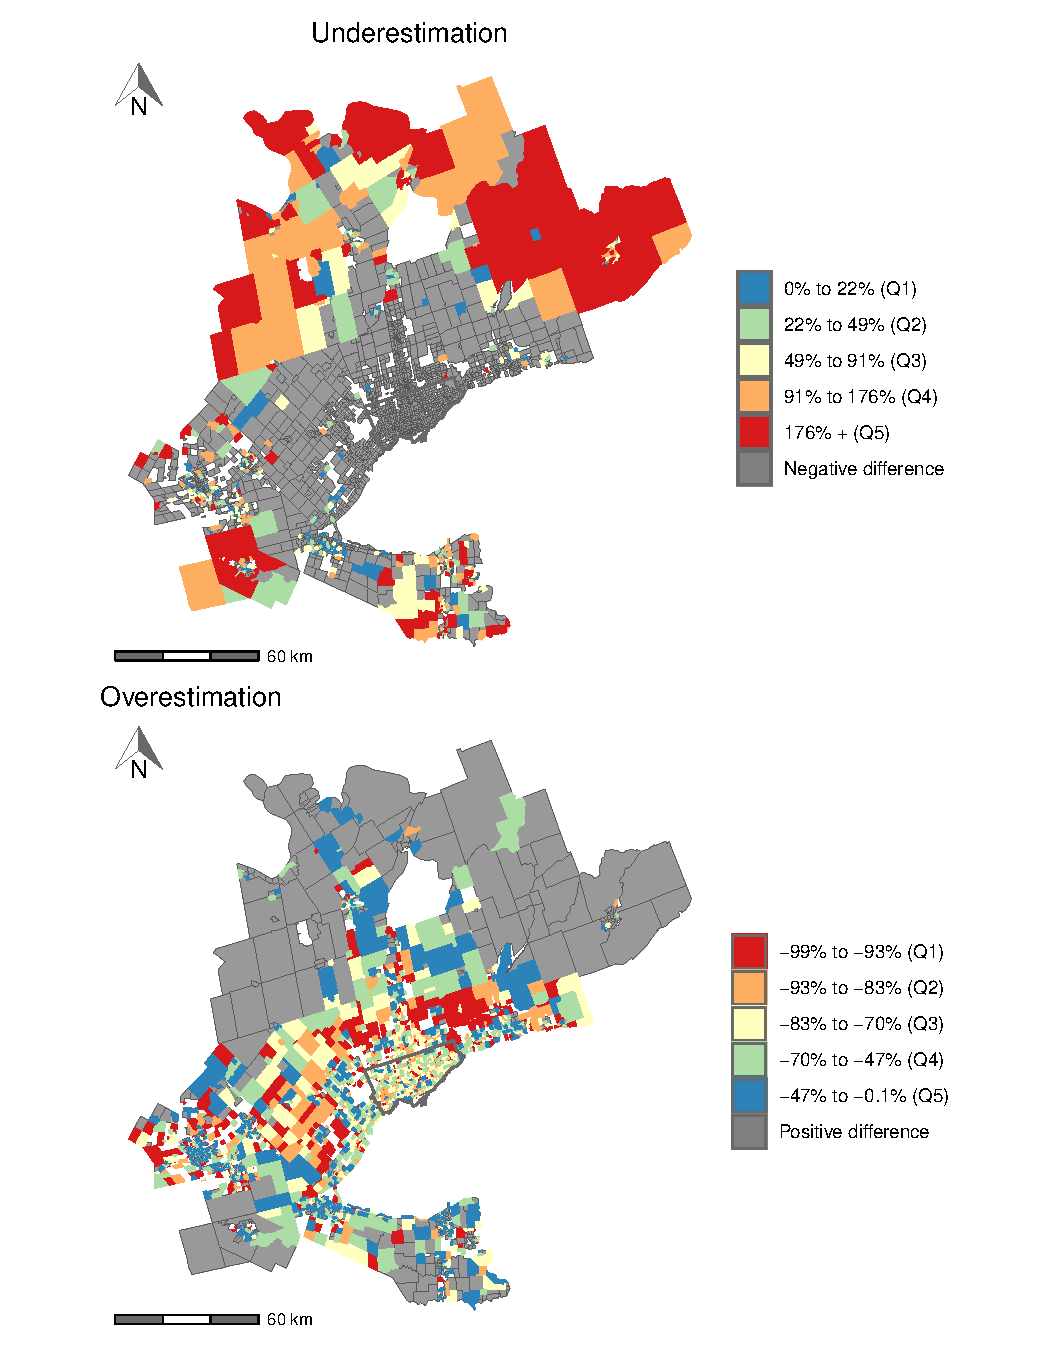
\includegraphics[width=1\linewidth]{Spatial-Availability_files/figure-latex/plot-difference-GGH-1} \caption{\label{fig:plot-difference-GGH}Difference between re-scaled the accessibility and the spatial availability job access measure in the context of employment from origins in the GGH to destinations in the City of Toronto. Values are expressed in five quantile ranges. Vivid TAZs represent a significant spatial autocorrelation and dimmed TAZs represent a non-signficant autocorrelation as measured by Local Moran's I only for underestimated TAZs. TAZs with values which are higher than re-scaled accessibility (positive difference) are shown fully in grey.}\label{fig:plot-difference-GGH}
\end{figure}

As observed from Figure \ref{fig:plot-difference-GGH}, TAZ with
underestimated job access (i.e., re-scaled accessibility values are
smaller than re-scaled spatial availability values) are located on the
periphery of the GGH area. The majority of these underestimated TAZ are
not within the center of the GGH where the city of Toronto and the
Greater Toronto Area (GTA) is located but are in proximity to other,
smaller, employment areas within smaller municipalities . It can be
understood that the underestimation of TAZ is a result of both high
spatial availability as a result of low job competition and low
accessibility scores that are a by-product of the job multiple-counting
occurring within more densely job-populated TAZ in the GTA.
Accessibility's multiple-counting effectively deflates the job access in
these peripheral TAZ since their accessibility values are significantly
lower compared to their multiple-counted GTA TAZ neighbours. The impact
of this multiple-counting is starkly apparent when compared to the
re-scaled spatial availability measure since spatial availability
allocates jobs proportionally based on workers and travel cost, TAZ do
not multiple-counting of jobs and TAZ which are not in the position to
multiple-count are not deflated as a consequence . This is supported by
viewing the spatial availability of jobs per capita (Figure
\ref{fig:plot-avail-GGH-TTS-per-worker}) where we can see that
commercial areas throughout the GGH have similar job access values as
within some commercial areas in the GTA; this is not the case for the
accessibility measure (see trends in Figure
\ref{fig:plot-access-SA-GGH-TTS}).

Next, it is worth explaining why accessibility's multiple counting does
not also result in the underestimation of job access when considering
only considering the jobs available in Toronto. As depicted in the
previous Figure \ref{fig:plot-local-i-Toronto}, almost all TAZ are
overestimates (i.e., accessibility values are \emph{higher} than spatial
availability). Within this subset of jobs in these peripheral TAZ,
spatial availability is proportionally allocated based on their high
(compared to the region) travel cost and Toronto-working population. In
essence, these TAZ experience moderately high job competition and thus
have low spatial availability. When accessibility is calculated, these
peripheral TAZ have low accessibility as a result of the
multiple-counting which occurs within and around Toronto but when the
two measures are compared, however, accessibility is still \emph{higher}
than spatial availability. The difference in the two measures flips when
the workers who work in areas outside of Toronto are re-introduced to
these peripheral TAZ as represented in Figure
\ref{fig:plot-difference-GGH}. Since more workers (more competition) and
more jobs with lower travel costs (less competition) are introduced, it
can be inferred that these peripheral TAZ experience moderately higher
job access (compare spatial availability per capita within these
periphery TAZ in Figure \ref{fig:plot-avail-Toronto-TTS-per-worker} and
Figure \ref{fig:plot-avail-GGH-TTS-per-worker}). Conversely, for the
accessibility measure, the introduction of additional workers does not
meter the accessibility gained by the introduction of additional jobs
and as such, the re-scaled accessibility values are \emph{higher} than
than the spatial availability resulting in underestimated TAZ.

It is also worth noting that the right panel of Figure
\ref{fig:plot-difference-GGH}, by contrast, depicts all the TAZ with
overestimated job access (i.e., re-scaled accessibility values are
larger than re-scaled spatial availability values). Similar to the
difference between measures depicted in the previous Figure
\ref{fig:plot-local-i-Toronto} for the subset of jobs located in
Toronto, these TAZ which are mostly within the GTA reflect an increased
accessibility as a result of multiple-counting of jobs and a
comparatively low spatial availability as a result of high job
competition. Overall, within the full set of jobs in the GGH, the first
and second issue associated with accessibility's conglomeration effect
are observed.

\hypertarget{contextualizing-spatial-availability-use-cases}{%
\section{Contextualizing Spatial Availability Use
Cases}\label{contextualizing-spatial-availability-use-cases}}

In addition to measuring access to jobs for workers, spatial
availability can be used to measure many other opportunity types and
scenarios. In this section we demonstrate two additional ways in which
spatial availability can be applied. Since spatial availability
singly-constraints opportunities which are allocated to the demand
seeking population, opportunities or demand seeking populations can be
subset while the resulting access measure does not lose any
interpretability. As such, we firstly present a practical application is
calculating job access for a specialized subset of population to
specialized employment centers. We then present an application where the
roles of workers and employers are reversed and employers are the demand
seeking population. These two additional use cases are non-exhaust and
applications outside of employment are tenable and warranted.

To illustrate these two additional examples, we return to the toy data
set initially introduced in
\protect\hypertarget{background}{}{Background} section.

\hypertarget{available-jobs-for-specialized-working-populations}{%
\subsection{Available Jobs for Specialized Working
Populations}\label{available-jobs-for-specialized-working-populations}}

Suppose that population centers 1 through 8 are not all eligible for
employment at the three employment centers 1, 2, and 3. This can be due
to education attainment or more simply a geographic barrier (i.e., river
without a road) making it impossible for certain populations to be
employed at certain employment centers. In this toy data set, we
consider that only population center 1 and 2 are eligible for employment
at Employment Center 1. Next assume that jobs in employment center 2 can
be taken by individuals in population centers 3, 4, 5, 7, and 8. Lastly,
jobs in Employment Center 3 require qualifications available only among
individuals in population centers 5, 6, 8, and 9. In essence,
eligibility criteria create catchments which can be easily considered
within the spatial availability measure and this specialized job access
is presented in Figure
\ref{fig:toy-example-availability-with-catchments}.

\begin{figure}
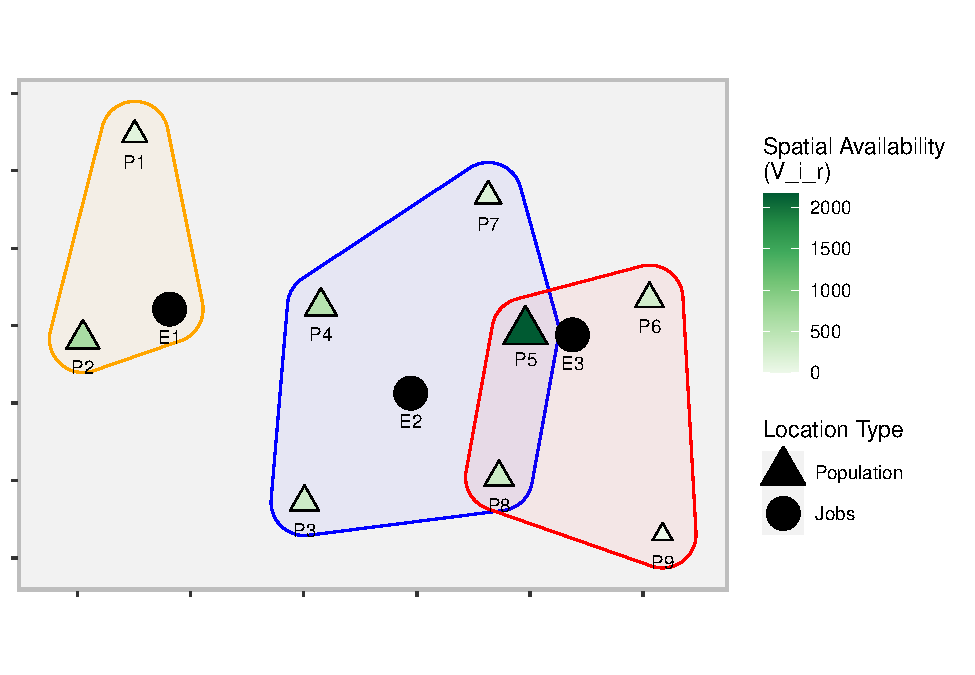
\includegraphics[width=1\linewidth]{Spatial-Availability_files/figure-latex/toy-example-availability-with-catchments-1} \caption{\label{fig:toy-example-availability-with-catchments}Spatial availability of jobs from population centers assuming catchment restrictions for the simple toy data set}\label{fig:toy-example-availability-with-catchments}
\end{figure}

\begin{figure}
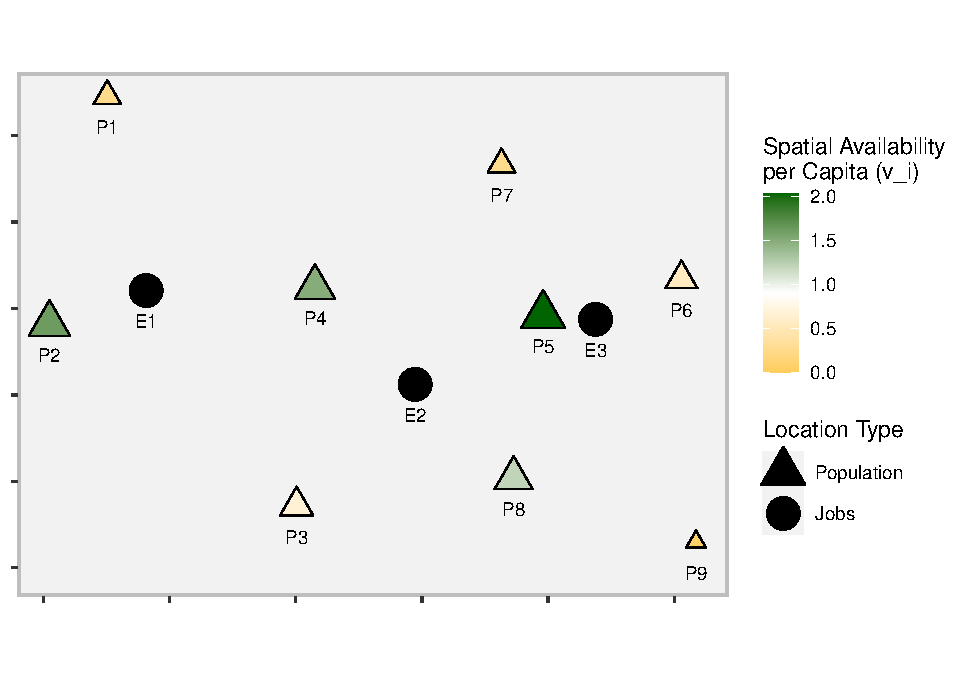
\includegraphics[width=1\linewidth]{Spatial-Availability_files/figure-latex/toy-example-availability-jobs-per-capita-1} \caption{\label{fig:toy-example-availability-jobs-per-capita} Spatial availability of jobs per capita for each population centers with catchment restrictions (top) and without catchment restrictions (bottom) for the simple toy data set}\label{fig:toy-example-availability-jobs-per-capita}
\end{figure}

For higher interpretability, we can view Figure
\ref{fig:toy-example-availability-jobs-per-capita} which demonstrates a
plot of spatial availability per captia considering catchments and also
another plot which assumes the same number of employment center
opportunities and population but no catchments.

In the bottom plot of Figure
\ref{fig:toy-example-availability-jobs-per-capita}, we see that
population center 5 has the highest level of spatial availability, due
to being a large population center that is more relatively close to
jobs. We also see population centers which are further from employment
centers have low spatial availability (P1, P3, P6, P7, P9) and
population centers which are more central have, evidently, higher job
access. We can also discern that the regional spatial availability per
capita is 0.908. In contrast, when catchments are introduced as shown in
the top plot of Figure
\ref{fig:toy-example-availability-jobs-per-capita}, we see that the job
access for population centers in the blue catchment decrease as job
competition increases. However, we also observe that access marginally
increases for the population centers in the yellow catchment and the
regional spatial availability per capita increases slightly to 0.964.

\hypertarget{alternative-use-case-3-available-workers-for-employment-centers}{%
\subsubsection{Alternative Use Case 3: Available Workers for Employment
Centers}\label{alternative-use-case-3-available-workers-for-employment-centers}}

Moving away from catchments in this next use case, we can easily switch
the demand and opportunity roles of the employment centers and
population centers. In this way, this use cases examines the pool of
workers available (demand) to each employment center by considering the
workers as the opportunities. We caculate spatial availability in the
same way by proportionally allocating jobs to workers based on travel
cost and numbers of jobs. Figure
\ref{fig:toy-example-availability-workers-per-job} presents the spatial
availability generally and per capita.

Plot the spatial availability of workers per job in Figure
\ref{fig:toy-example-availability-workers-per-job}

\begin{figure}
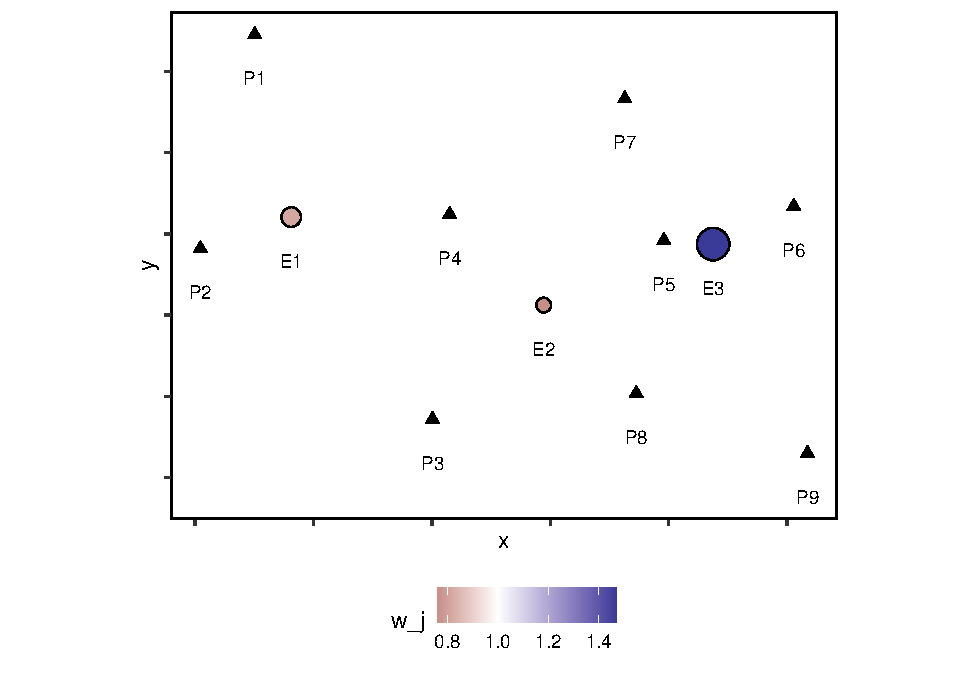
\includegraphics[width=1\linewidth]{Spatial-Availability_files/figure-latex/toy-example-availability-workers-per-job-1} \caption{\label{fig:toy-example-availability-workers-per-job} Spatial availability of workers for each employment center (top) and the spatial availability of workers per job for each employment center (bottom) for the simple toy data set}\label{fig:toy-example-availability-workers-per-job}
\end{figure}

\hypertarget{conclusing-remarks}{%
\section{Conclusing remarks}\label{conclusing-remarks}}

we argue that the proposed measure offers higher interpretability as it
opportunity per capita values can be derived to benchmark regional
results and per capita values can be compared across regions more
meaningfully.

Words go here.

still does not tell us how many accessible opportunities will lead to
participation/positive outcomes; it does come closer\ldots{} this is an
important question for equity analysis.

we propose that spatial availability be seen as a type of \emph{spatial
mismatch} and an evolution of the \emph{balanced floating catchment}
approach (BFCA) . Historically, literature has iteratively improved
measures assessing access to opportunities. In the context of employment
and healthcare opportunities, simple container counting solutions such
as the population-to-provider ratio (PPR) for healthcare services and
jobs to housing ratio were implemented. This approach, while straight
forward, is highly suspitable to the modifiable unit area problem
(MUAP). Recognizing this and harnessing the computation power and access
to finer resolution data as it became available, scholars proposed the
next evolution, namely the accessibility measure which is widely used
today and we implemented in our examples for comparison. It partially
addresses the MUAP by considering opportunities outside of the
conventional `containers' which represented opportunities in a census
areas/neighbourhoods by counting opportunities informed by an impedance
function based on travel cost. Our measure, spatial availability,
iterates on the accessibility measure by proportionally allocating
travel cost and population (workers) of origins to opportunities at
destinations. This single-constrained approach ensures that the
population is mutually exclusive in essence replicating the properties
of the self-contained unit which is \emph{not} limited to a zoning
system proposed; the pros of accessibility solution in using the
impedance function and pros of the container solutions.

Similar to the accessibility measure, it should be noted that spatial
availability is only as robust to the MUAP as the input data allows. For
instance, in the empirical example present, the measure of \emph{job
access} still only considers population, opportunities, and travel times
from the centroids of TAZs. However, unlike the accessibility measure,
spatial availability can be meaningful calculated on a per population
basis at higher resolutions because of the proportionality property.

Further, the measure of spatial availability can be a useful way to
distinguish between low accessibility/low population centers, which may
enjoy higher availability than the accessibility value may suggest, and
contrariwise, high accessibility/high population centers (which
potentially can result in lower availability due to competition). For
instance, as presented in the toy data set, more remote, smaller
population centers can have sufficient spatial availability by being in
close proximity to the smaller employment centers; however this
sufficiency is obscured by accessibility measure by conglomerating
accessibly of population centers which are more central to more (and
larger) employment centers. Conversely, referring to the empirical GGH
example, the TAZs that are relatively close to the Toronto job
destinations but have a relatively low number of workers receive
sufficiently high values of accessibility and signficantly lower spatial
availability values; this trend is opposite to what is experienced in
the toy data set and is a result of higher job competition (i.e.~job
opportunities are more highly allocated to TAZs with lower travel costs
and higher worker populations). Measuring access to opportunities is a
multi-scale problem; since the number of opportunities are preserved,
different scales, populations, and time-windows can be incorporated
within the measure without introducing additional spatial basis.

Fundamentally, accessibility measure's methodology results in the
overestimation of \emph{jobs access} since it simply sums the count of
destination opportunities based on travel cost to opportunities; the
measure does not include factors to bound the summation so origins,
hypothetically, can have infinite \emph{opportunity access}. This
property can be practical for calculating \emph{opportunity access} for
opportunities which have large capacities and are \emph{non-competitive}
such as large natural parks and beaches. These non-competitive
opportunities can be considered infinitely divisible as they offer more
`spots' at any given time than the population. However, often times
opportunities are not divisible but are in fact indivisible and
competitive meaning, such as the numerical and GGH empirical example of
\emph{jobs access}, where only 1 worker can access 1 job at any given
time. In these cases, spatial availability measure can be used to
calculate the \emph{opportunity access} in which the report values are
numerically meaningful, the MUAP is potentially addressed, and
\emph{opportunity access} values across regions, neighbourhoods, and
spatial scales can be compared.

\hypertarget{appendix}{%
\section{Appendix}\label{appendix}}

\begin{figure}
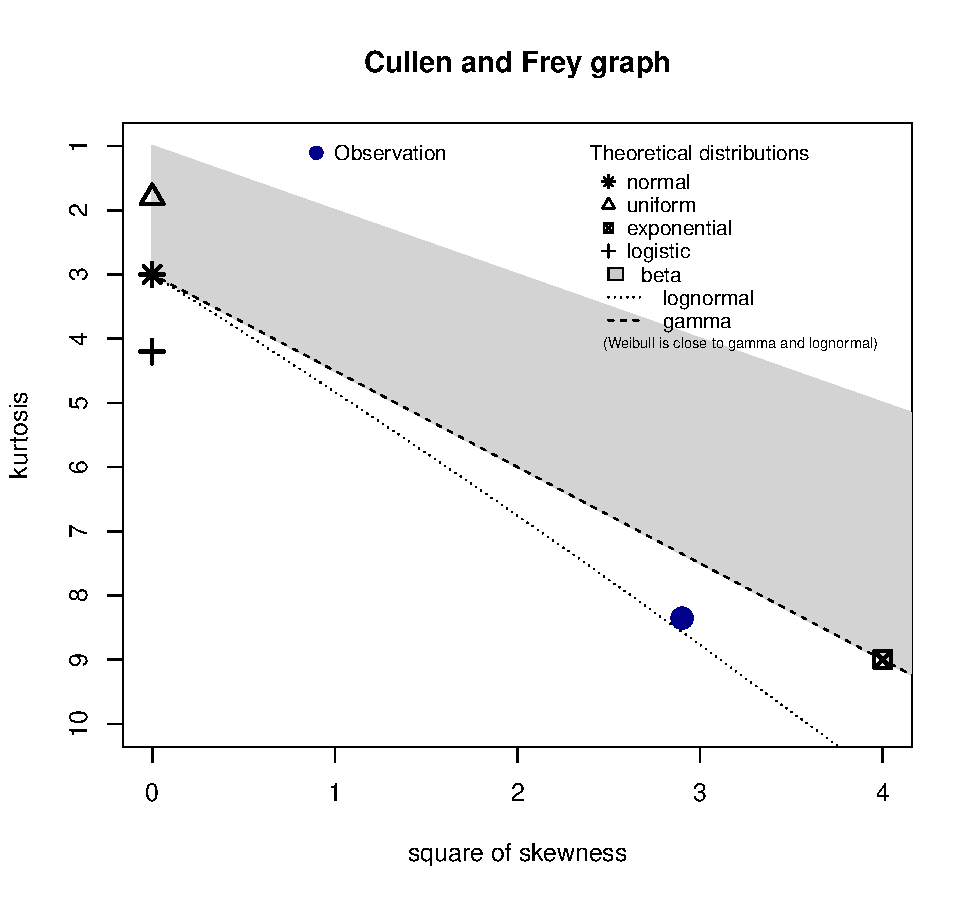
\includegraphics[width=1\linewidth]{Spatial-Availability_files/figure-latex/plot-cullen-frey-1} \caption{\label{fig:plot-cullen-frey}Cullen and frey graphy for the complete empirical 2016 TTS travel time data set.}\label{fig:plot-cullen-frey}
\end{figure}

\begin{verbatim}
summary statistics
------
min:  0.1   max:  179 
median:  18 
mean:  21.4344 
estimated sd:  14.61254 
estimated skewness:  1.703326 
estimated kurtosis:  8.353363 
\end{verbatim}

\begin{figure}
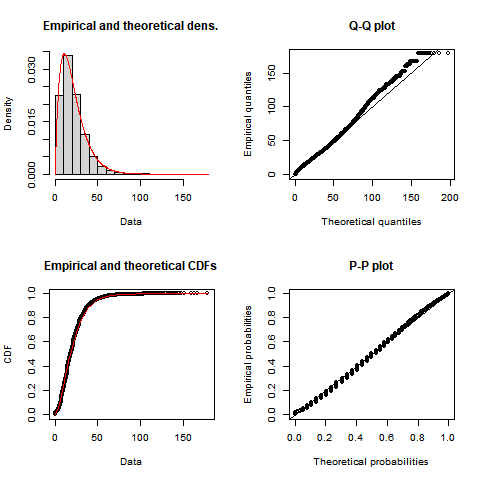
\includegraphics[width=1\linewidth]{images/impedance_function} \caption{\label{fig:impedance-function-plot}Diagnostics associated with the fitted gamma distribution.}\label{fig:plot-impedance-function}
\end{figure}

\hypertarget{references}{%
\section*{References}\label{references}}
\addcontentsline{toc}{section}{References}

\hypertarget{refs}{}
\begin{CSLReferences}{1}{0}
\leavevmode\vadjust pre{\hypertarget{ref-allen2019}{}}%
Allen, J., Farber, S., 2019. A Measure of Competitive Access to
Destinations for Comparing Across Multiple Study Regions. Geographical
Analysis 52, 69--86.
doi:\href{https://doi.org/10.1111/gean.12188}{10.1111/gean.12188}

\leavevmode\vadjust pre{\hypertarget{ref-anselin1995local}{}}%
Anselin, L., 1995. Local indicators of spatial association - LISA.
Geographical Analysis 27, 93--115.

\leavevmode\vadjust pre{\hypertarget{ref-deboosere2018}{}}%
Deboosere, R., El-Geneidy, A.M., Levinson, D., 2018.
Accessibility-oriented development. Journal of Transport Geography 70,
11--20.
doi:\href{https://doi.org/10.1016/j.jtrangeo.2018.05.015}{10.1016/j.jtrangeo.2018.05.015}

\leavevmode\vadjust pre{\hypertarget{ref-delamater2013spatial}{}}%
Delamater, P.L., 2013. Spatial accessibility in suboptimally configured
health care systems: A modified two-step floating catchment area
(M2SFCA) metric. Health \& Place 24, 30--43.
doi:\href{https://doi.org/10.1016/j.healthplace.2013.07.012}{10.1016/j.healthplace.2013.07.012}

\leavevmode\vadjust pre{\hypertarget{ref-fitdistrplus_2015}{}}%
Delignette-Muller, M.L., Dutang, C., 2015. {fitdistrplus}: An {R}
package for fitting distributions. Journal of Statistical Software 64,
1--34.

\leavevmode\vadjust pre{\hypertarget{ref-geurs2004}{}}%
Geurs, K.T., van Wee, B., 2004. Accessibility evaluation of land-use and
transport strategies: review and research directions. Journal of
Transport Geography 12, 127--140.
doi:\href{https://doi.org/10.1016/j.jtrangeo.2003.10.005}{10.1016/j.jtrangeo.2003.10.005}

\leavevmode\vadjust pre{\hypertarget{ref-handy2020}{}}%
Handy, S., 2020. Is accessibility an idea whose time has finally come?
Transportation Research Part D: Transport and Environment 83, 102319.
doi:\href{https://doi.org/10.1016/j.trd.2020.102319}{10.1016/j.trd.2020.102319}

\leavevmode\vadjust pre{\hypertarget{ref-hansen1959}{}}%
Hansen, W.G., 1959. How Accessibility Shapes Land Use. Journal of the
American Institute of Planners 25, 73--76.
doi:\href{https://doi.org/10.1080/01944365908978307}{10.1080/01944365908978307}

\leavevmode\vadjust pre{\hypertarget{ref-joseph1984}{}}%
Joseph, A.E., Bantock, P.R., 1984. Rural Accessibility of General
Practitioners: the Case of Bruce and Grey Counties, ONTARIO,
1901{\textendash}1981. The Canadian Geographer/Le Géographe canadien 28,
226--239.
doi:\href{https://doi.org/10.1111/j.1541-0064.1984.tb00788.x}{10.1111/j.1541-0064.1984.tb00788.x}

\leavevmode\vadjust pre{\hypertarget{ref-luo2003}{}}%
Luo, W., Wang, F., 2003. Measures of Spatial Accessibility to Health
Care in a GIS Environment: Synthesis and a Case Study in the Chicago
Region. Environment and Planning B: Planning and Design 30, 865--884.
doi:\href{https://doi.org/10.1068/b29120}{10.1068/b29120}

\leavevmode\vadjust pre{\hypertarget{ref-miller2018}{}}%
Miller, E.J., 2018. Accessibility: measurement and application in
transportation planning. Transport Reviews 38, 551--555.
doi:\href{https://doi.org/10.1080/01441647.2018.1492778}{10.1080/01441647.2018.1492778}

\leavevmode\vadjust pre{\hypertarget{ref-paez2019}{}}%
Paez, A., Higgins, C.D., Vivona, S.F., 2019. Demand and level of service
inflation in Floating Catchment Area (FCA) methods. PLOS ONE 14,
e0218773.
doi:\href{https://doi.org/10.1371/journal.pone.0218773}{10.1371/journal.pone.0218773}

\leavevmode\vadjust pre{\hypertarget{ref-proffitt2017}{}}%
Proffitt, D.G., Bartholomew, K., Ewing, R., Miller, H.J., 2017.
Accessibility planning in American metropolitan areas: Are we there yet?
Urban Studies 56, 167--192.
doi:\href{https://doi.org/10.1177/0042098017710122}{10.1177/0042098017710122}

\leavevmode\vadjust pre{\hypertarget{ref-r5r_2021}{}}%
Rafael H. M. Pereira, Marcus Saraiva, Daniel Herszenhut, Carlos Kaue
Vieira Braga, Matthew Wigginton Conway, 2021. r5r: Rapid realistic
routing on multimodal transport networks with R5 in r. Findings.
doi:\href{https://doi.org/10.32866/001c.21262}{10.32866/001c.21262}

\leavevmode\vadjust pre{\hypertarget{ref-shen1998}{}}%
Shen, Q., 1998. Location characteristics of inner-city neighborhoods and
employment accessibility of low-wage workers. Environment and Planning
B: Planning and Design 25, 345--365.
doi:\href{https://doi.org/10.1068/b250345}{10.1068/b250345}

\leavevmode\vadjust pre{\hypertarget{ref-wan2012three}{}}%
Wan, N., Zou, B., Sternberg, T., 2012. A three-step floating catchment
area method for analyzing spatial access to health services.
International Journal of Geographical Information Science 26,
1073--1089.
doi:\href{https://doi.org/10.1080/13658816.2011.624987}{10.1080/13658816.2011.624987}

\leavevmode\vadjust pre{\hypertarget{ref-wilson1971}{}}%
Wilson, A.G., 1971. A Family of Spatial Interaction Models, and
Associated Developments. Environment and Planning A: Economy and Space
3, 1--32. doi:\href{https://doi.org/10.1068/a030001}{10.1068/a030001}

\leavevmode\vadjust pre{\hypertarget{ref-yan2021}{}}%
Yan, X., 2021. Toward Accessibility-Based Planning. Journal of the
American Planning Association 87, 409--423.
doi:\href{https://doi.org/10.1080/01944363.2020.1850321}{10.1080/01944363.2020.1850321}

\end{CSLReferences}


\end{document}
